\documentclass[../main.tex]{subfiles}
\graphicspath{{\subfix{../graphicsJCAT/}}}
\begin{document}

\begin{figure*}
\caption{Visual explanation of the inpainting method.}
\label{fig:inpainting_method_explanation}
\end{figure*}

\begin{figure*}
\caption{Visual explanation of the training of the GAN.}
\label{fig:training_procedure_explanation}
\end{figure*}

\subfile{graphicsJCAT/Figure3_SophiaBeadsSample.pdf}

\begin{figure*}
\subfloat[Sinogram with missing acquisitions drawn from the SophiaBeads dataset.]{\includegraphics[width=0.2\textwidth]{graphics/sophia_sin_example.png}
\label{fig:sophia_sin_example}}
\hspace{5mm}%
\subfloat[Mask associated with Fig. \ref{fig:sophia_sin_example}.]{\includegraphics[width=0.2\textwidth]{graphics/sophia_sin_mask.png}
\label{fig:sophia_sin_mask}}
\caption{Fig. \ref{fig:sophia_sin_example} shows a sinogram with missing acquisitions and Fig. \ref{fig:sophia_sin_mask} its associated mask.}
\label{fig:sinogram_example}
\end{figure*}
    
\begin{figure*}
\centering
\subfloat[Sample from the synthetic dataset.]{\includegraphics[width=0.2\textwidth]{graphics/syn_obj_slice.png}
\label{fig:syn_obj_slice}}
\hfil
\subfloat[Encoded shape prior associated to Fig. \ref{fig:syn_obj_slice}.]{\includegraphics[width=0.2\textwidth]{graphics/syn_cad_slice.png}
\label{fig:syn_cad_slice}}
\hfil
\subfloat[Sinogram corresponding to Fig. \ref{fig:syn_obj_slice}.]{\includegraphics[width=0.2\textwidth]{graphics/syn_obj_sin.png}
\label{fig:syn_obj_sin}}
\hfil
\subfloat[Sinogram corresponding to Fig. \ref{fig:syn_cad_slice}.]{\includegraphics[width=0.2\textwidth]{graphics/syn_cad_sin.png}
\label{fig:syn_cad_sin}}
\caption{Sample from the volume of the synthetic dataset. (\ref{fig:syn_obj_slice}) shows the ground-truth reconstruction and (\ref{fig:syn_cad_slice}) shows a representation of the shape priors showing each object with a different randomly assigned gray value, in which no plastic container is visible. In an attempt to reproduce noise in the image, a Gaussian noise is added to the material of uniform densities. The sinograms shown in (\ref{fig:syn_obj_sin}) and (\ref{fig:syn_cad_sin}) are obtained using the forward radon transform with a parallel beam geometry.}
        \label{fig:Sample synthetic}
\end{figure*}          

\begin{figure*}
\subfloat[Example of a sample of the synthetic dataset when internal defects are present.]{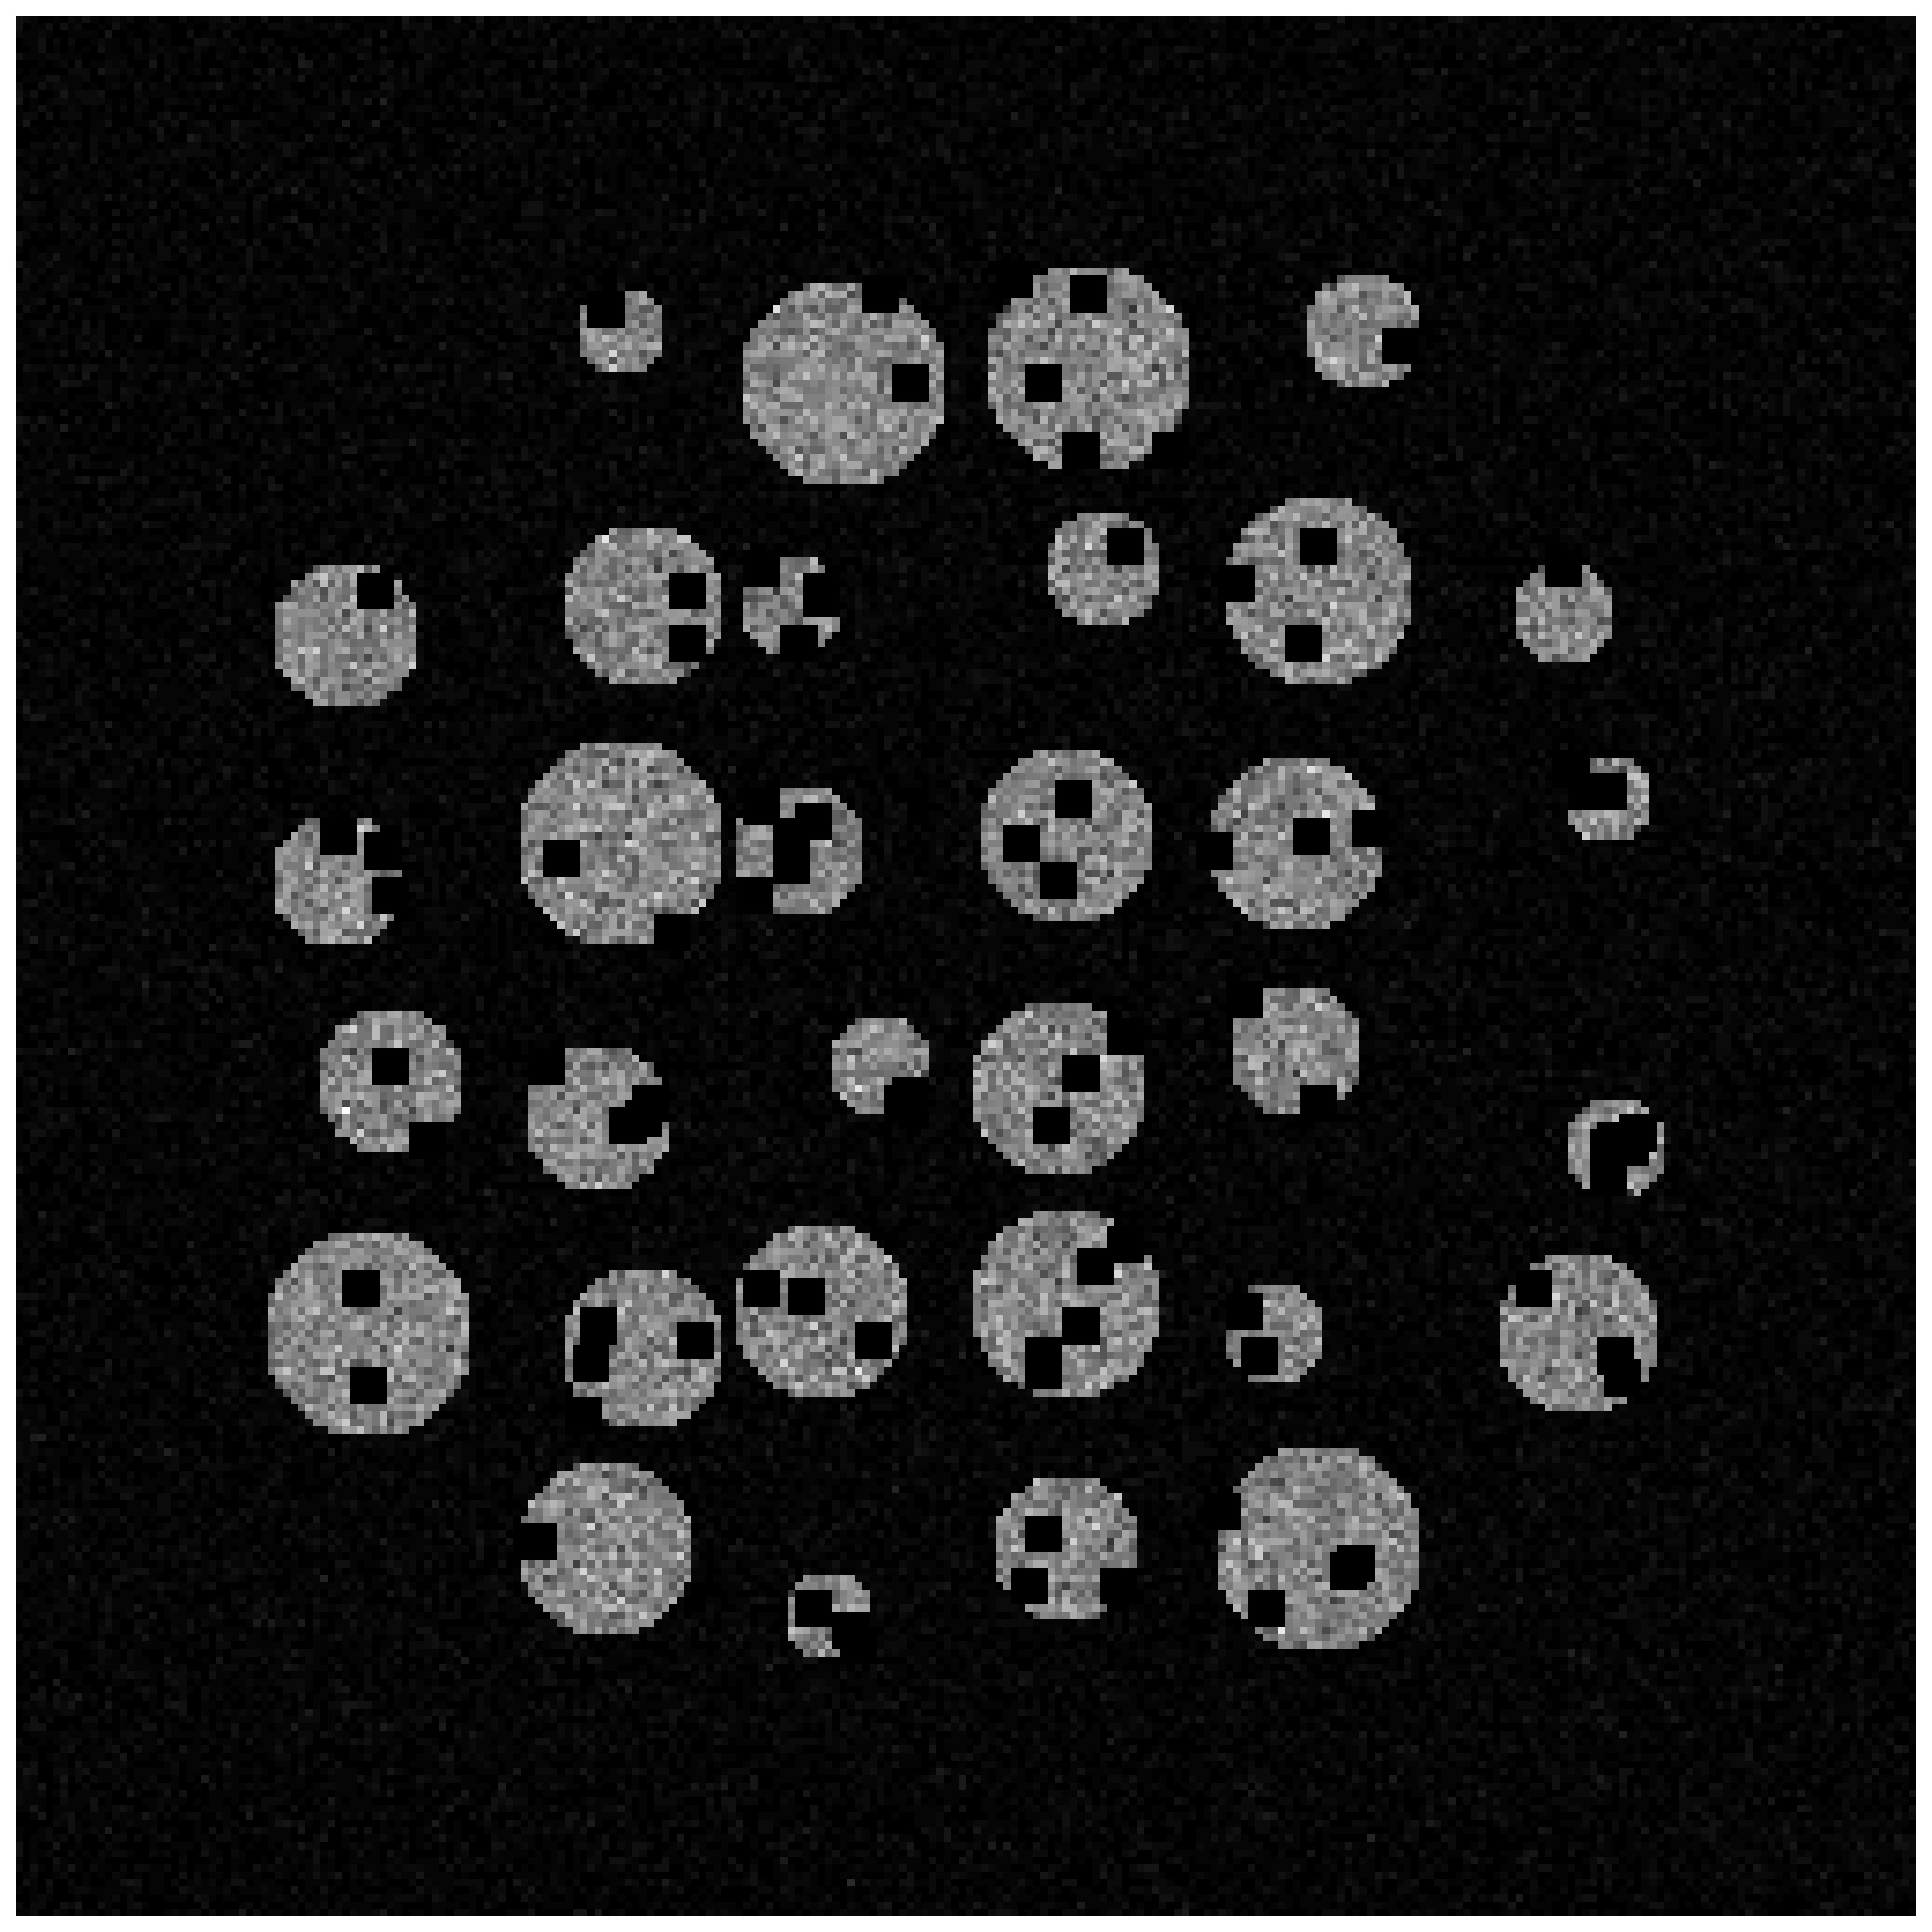
\includegraphics[width=0.2\textwidth]{graphics/syn_obj_holes_img.png}
\label{fig:holes_examples_}}
\caption{Objects with internal defects not encoded in the shape prior.}
\label{fig:holes_examples}
\end{figure*}

\begin{figure*}
\centering
\subfloat[Target reconstruction with 256 acquisitions]{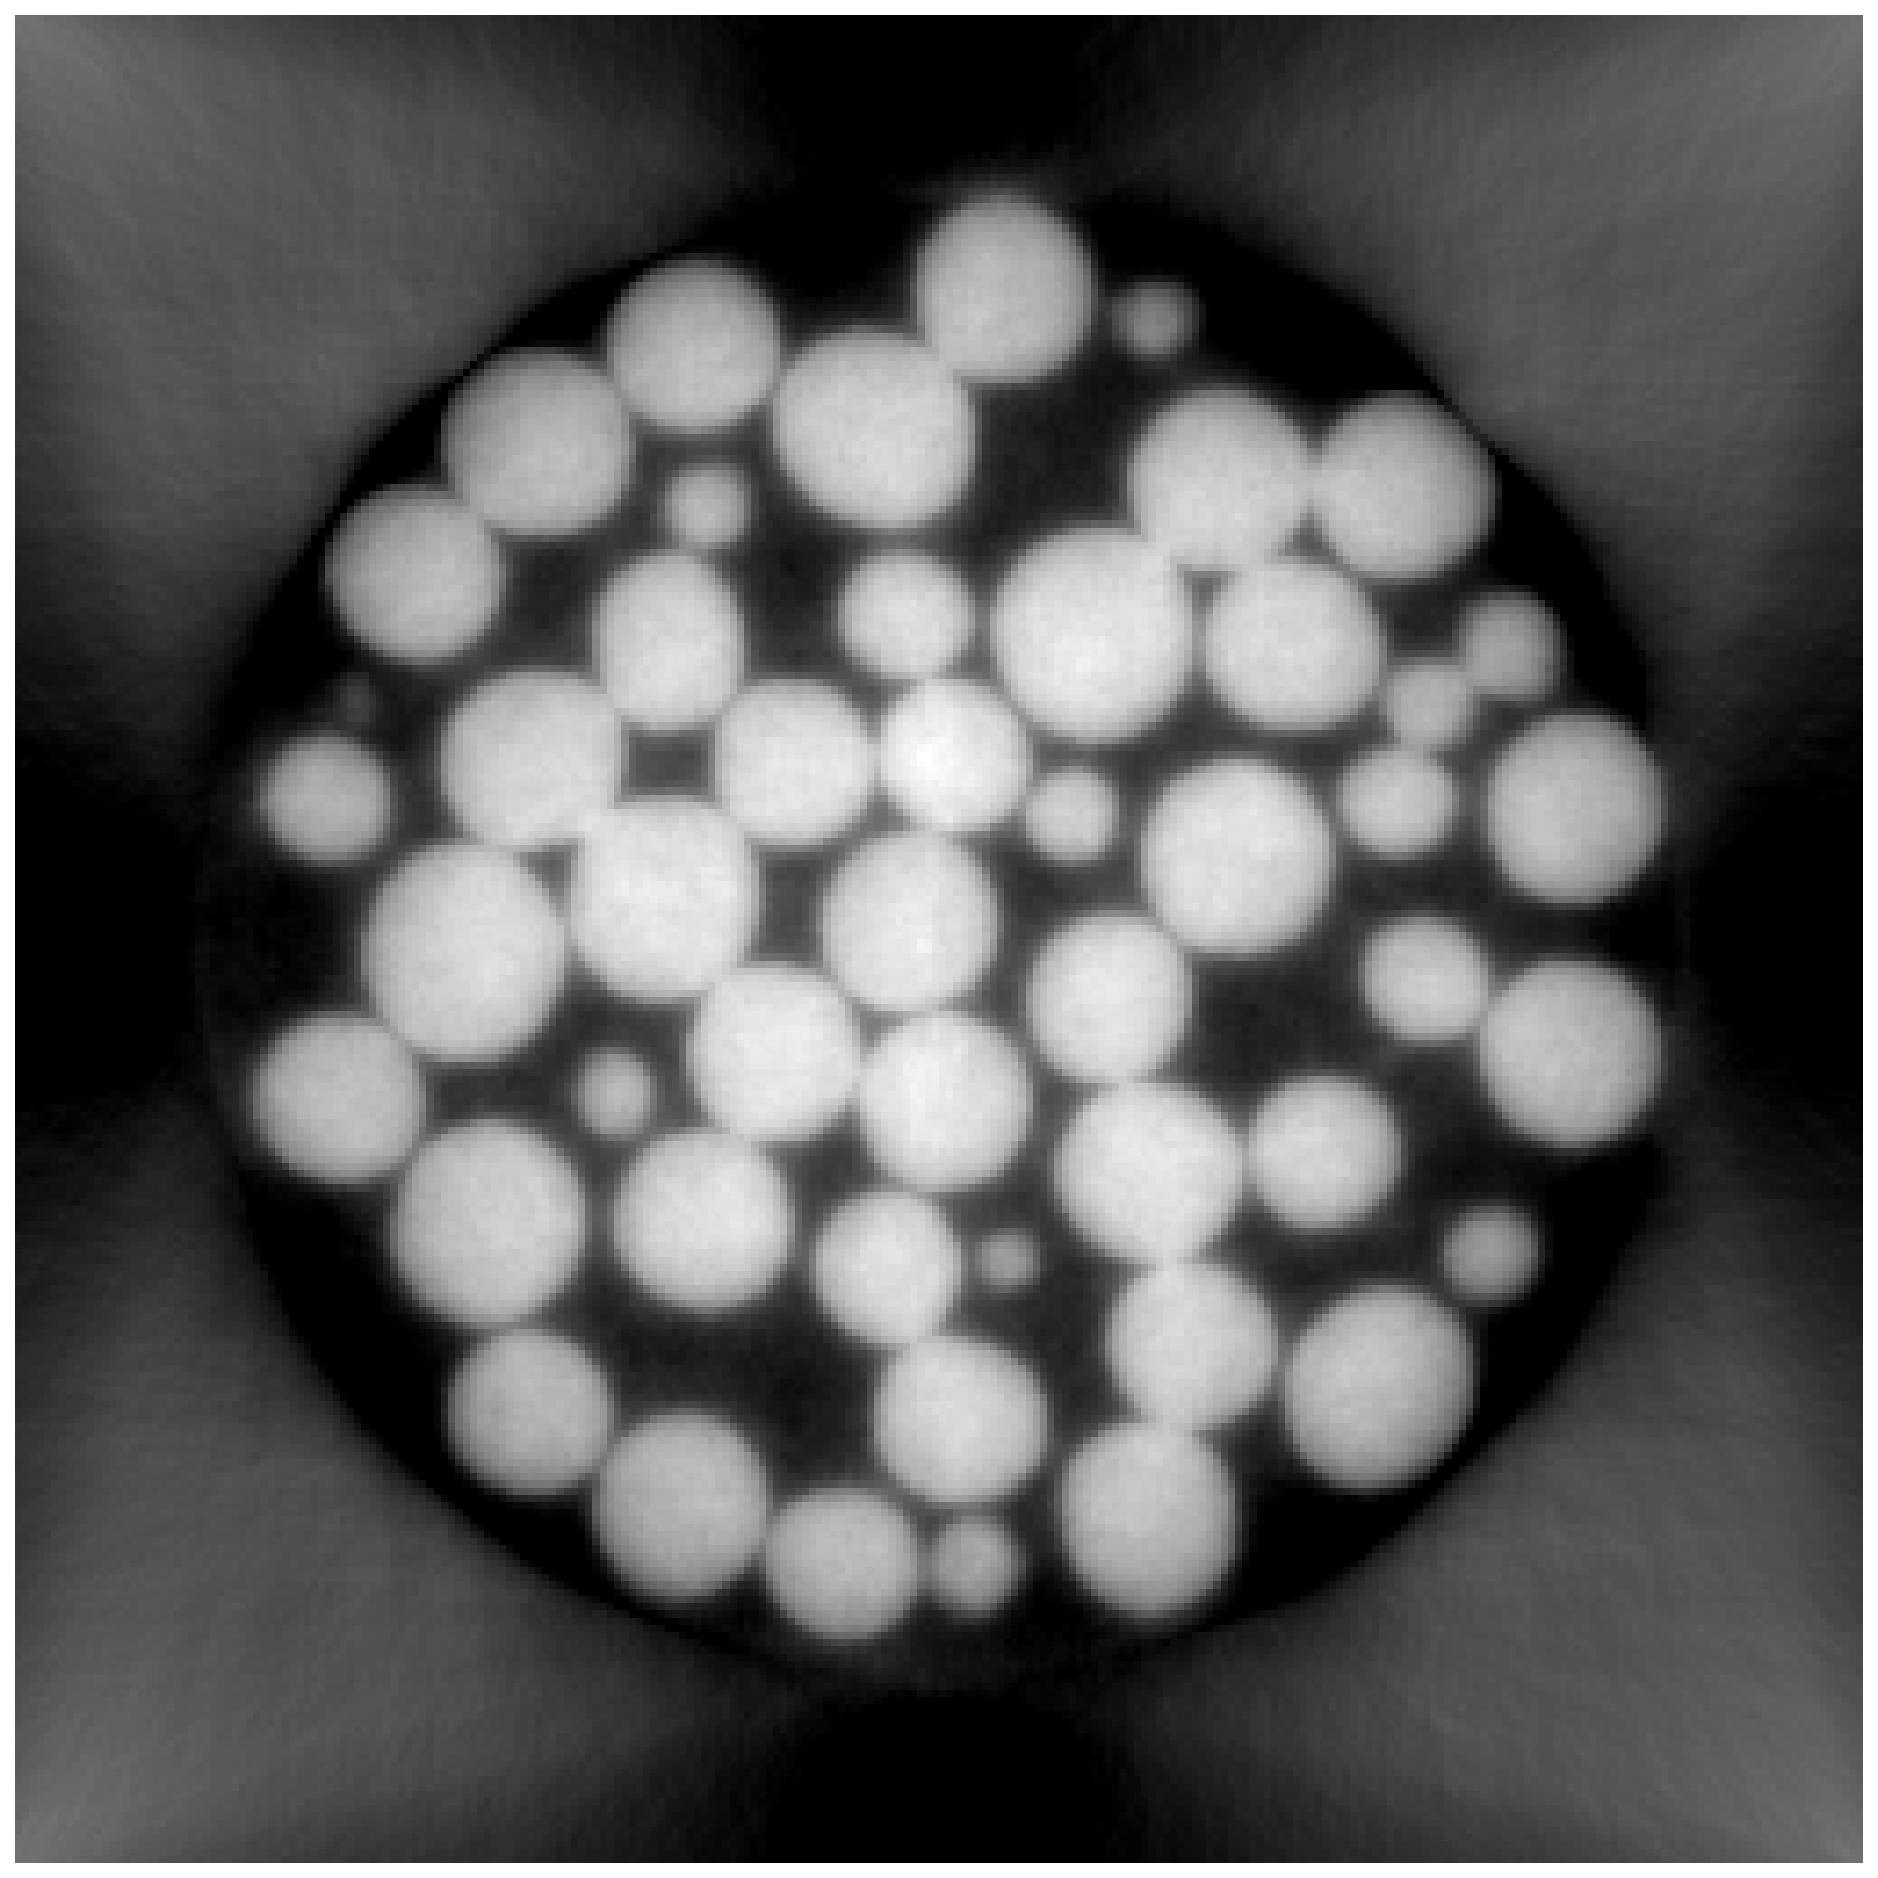
\includegraphics[width=0.2\textwidth]{graphics/reconstructions128_target.jpg}
\label{fig:reconstructions128_target}}
\hfill
\subfloat[Reconstruction without any interpolation method , i.e from 128 acquisitions]{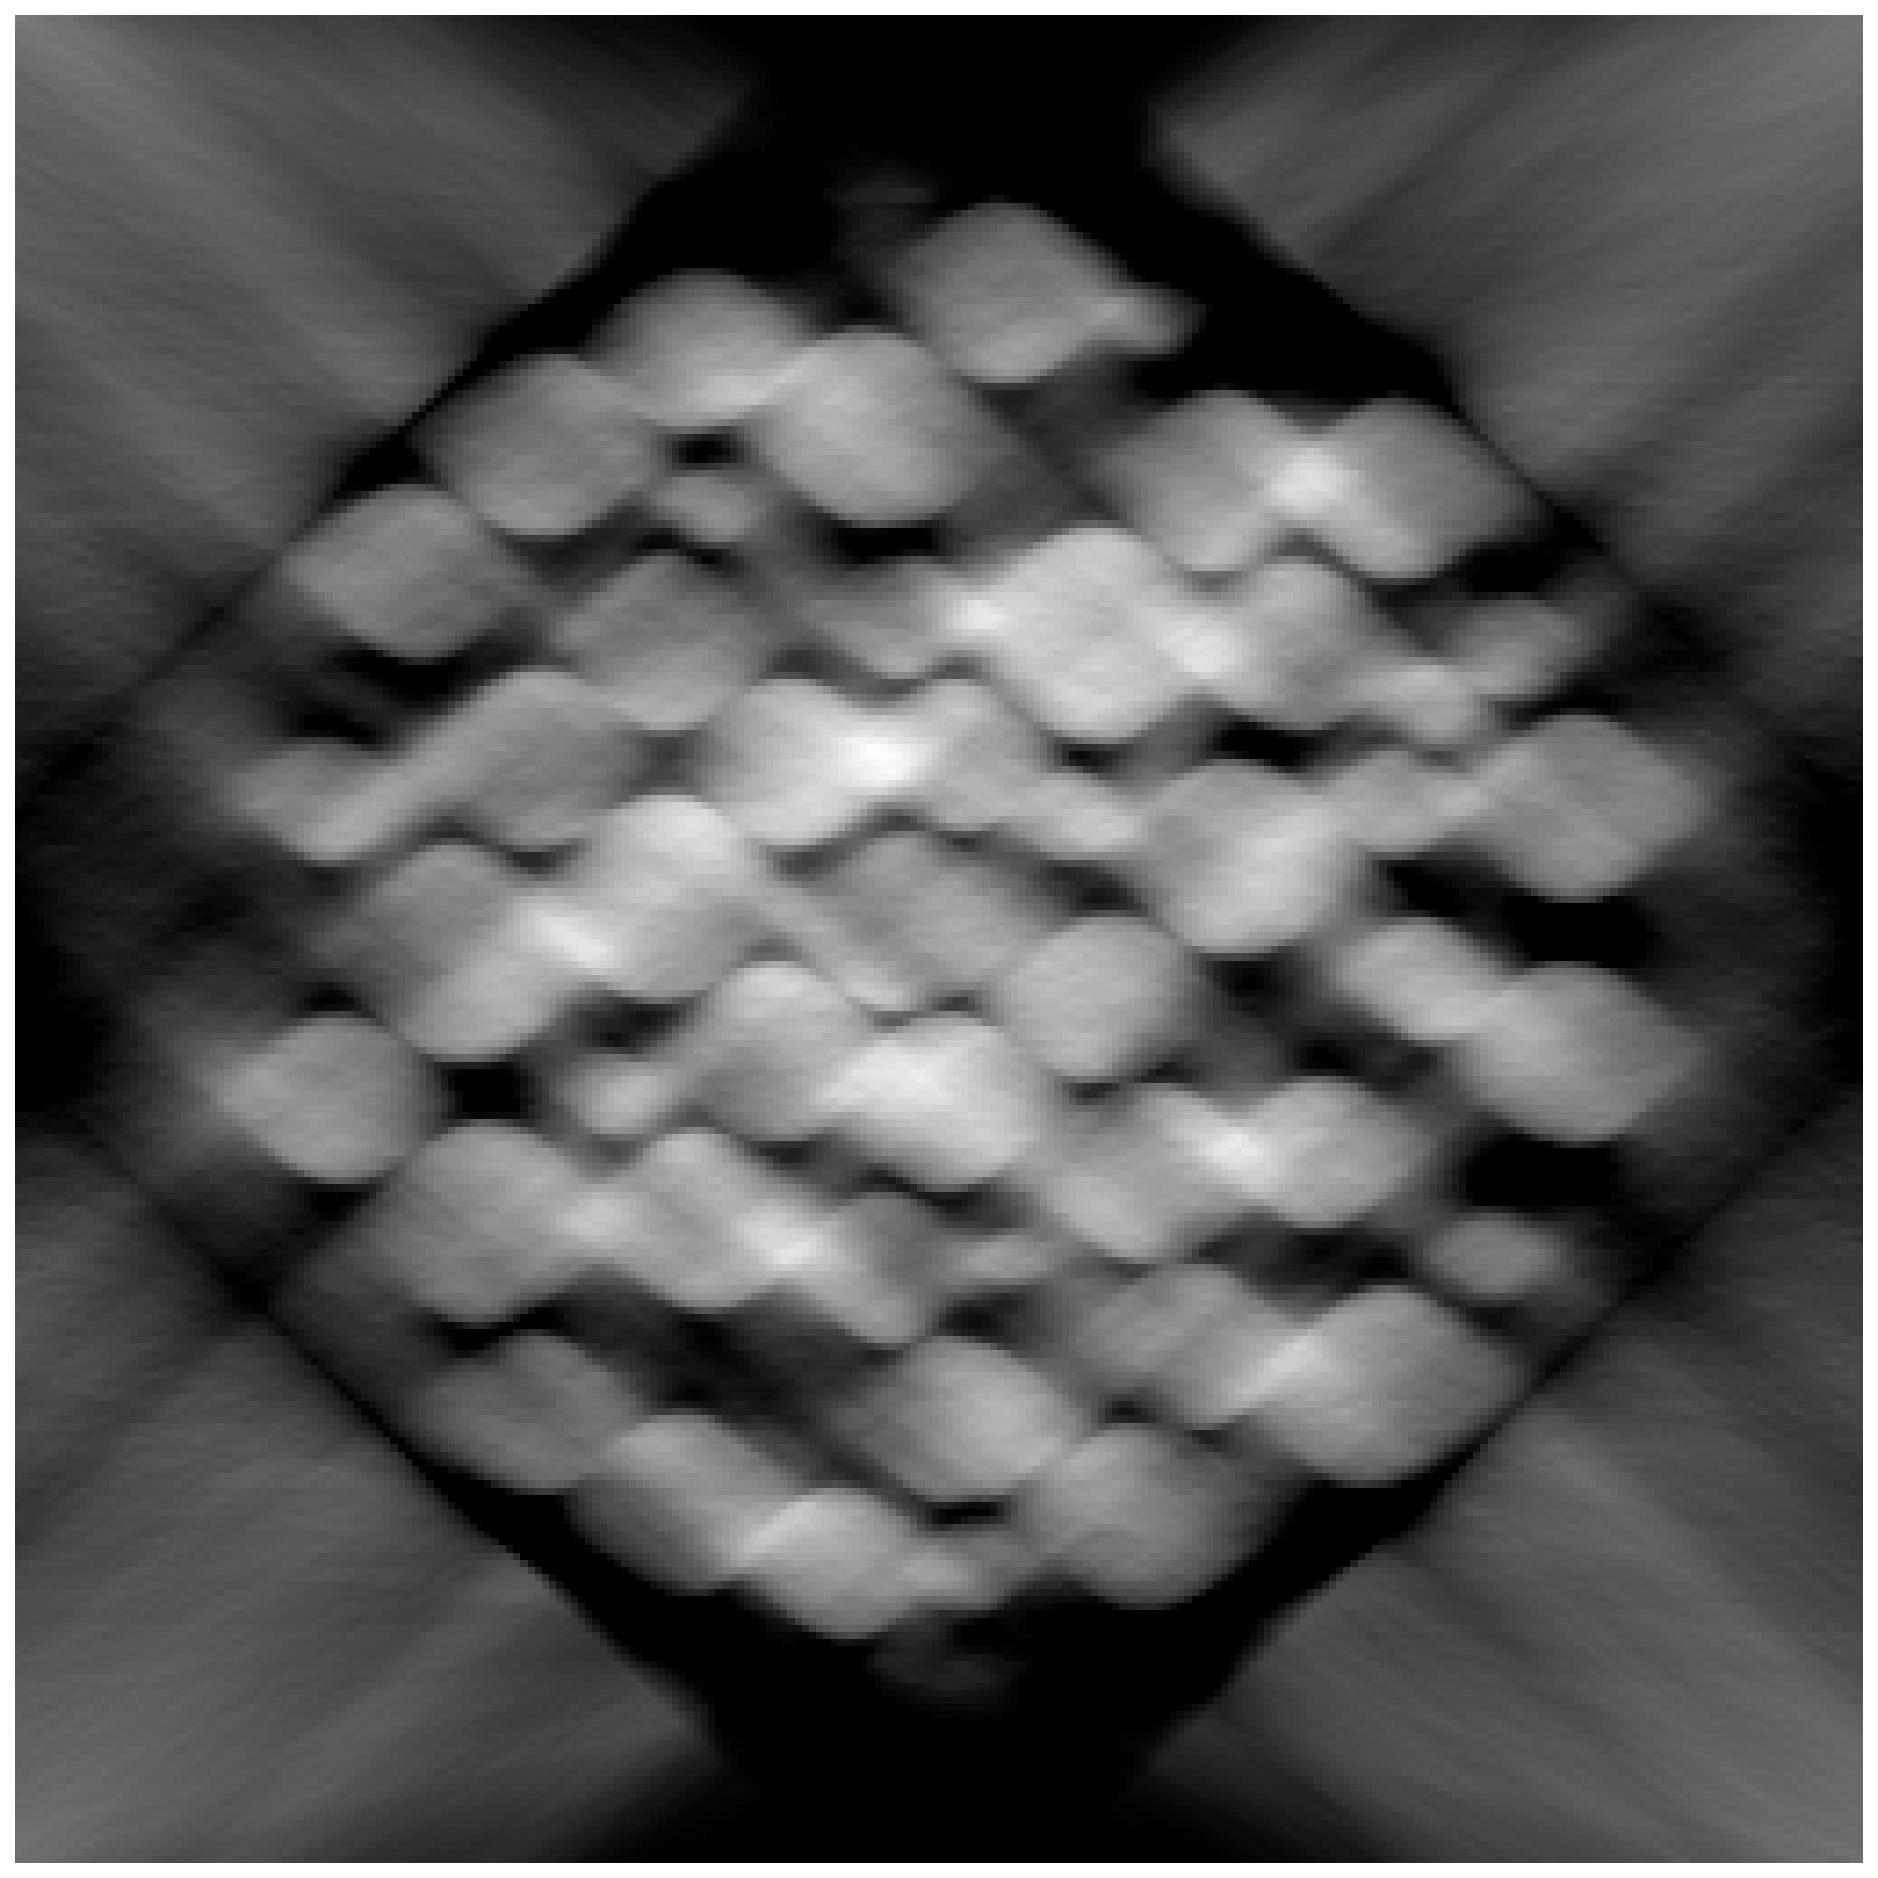
\includegraphics[width=0.2\textwidth]{graphics/reconstructions128_noInterpolation.jpg}
\label{fig:reconstructions128_noInterpolation}}
\hfill
\subfloat[Reconstruction with linear interpolation]{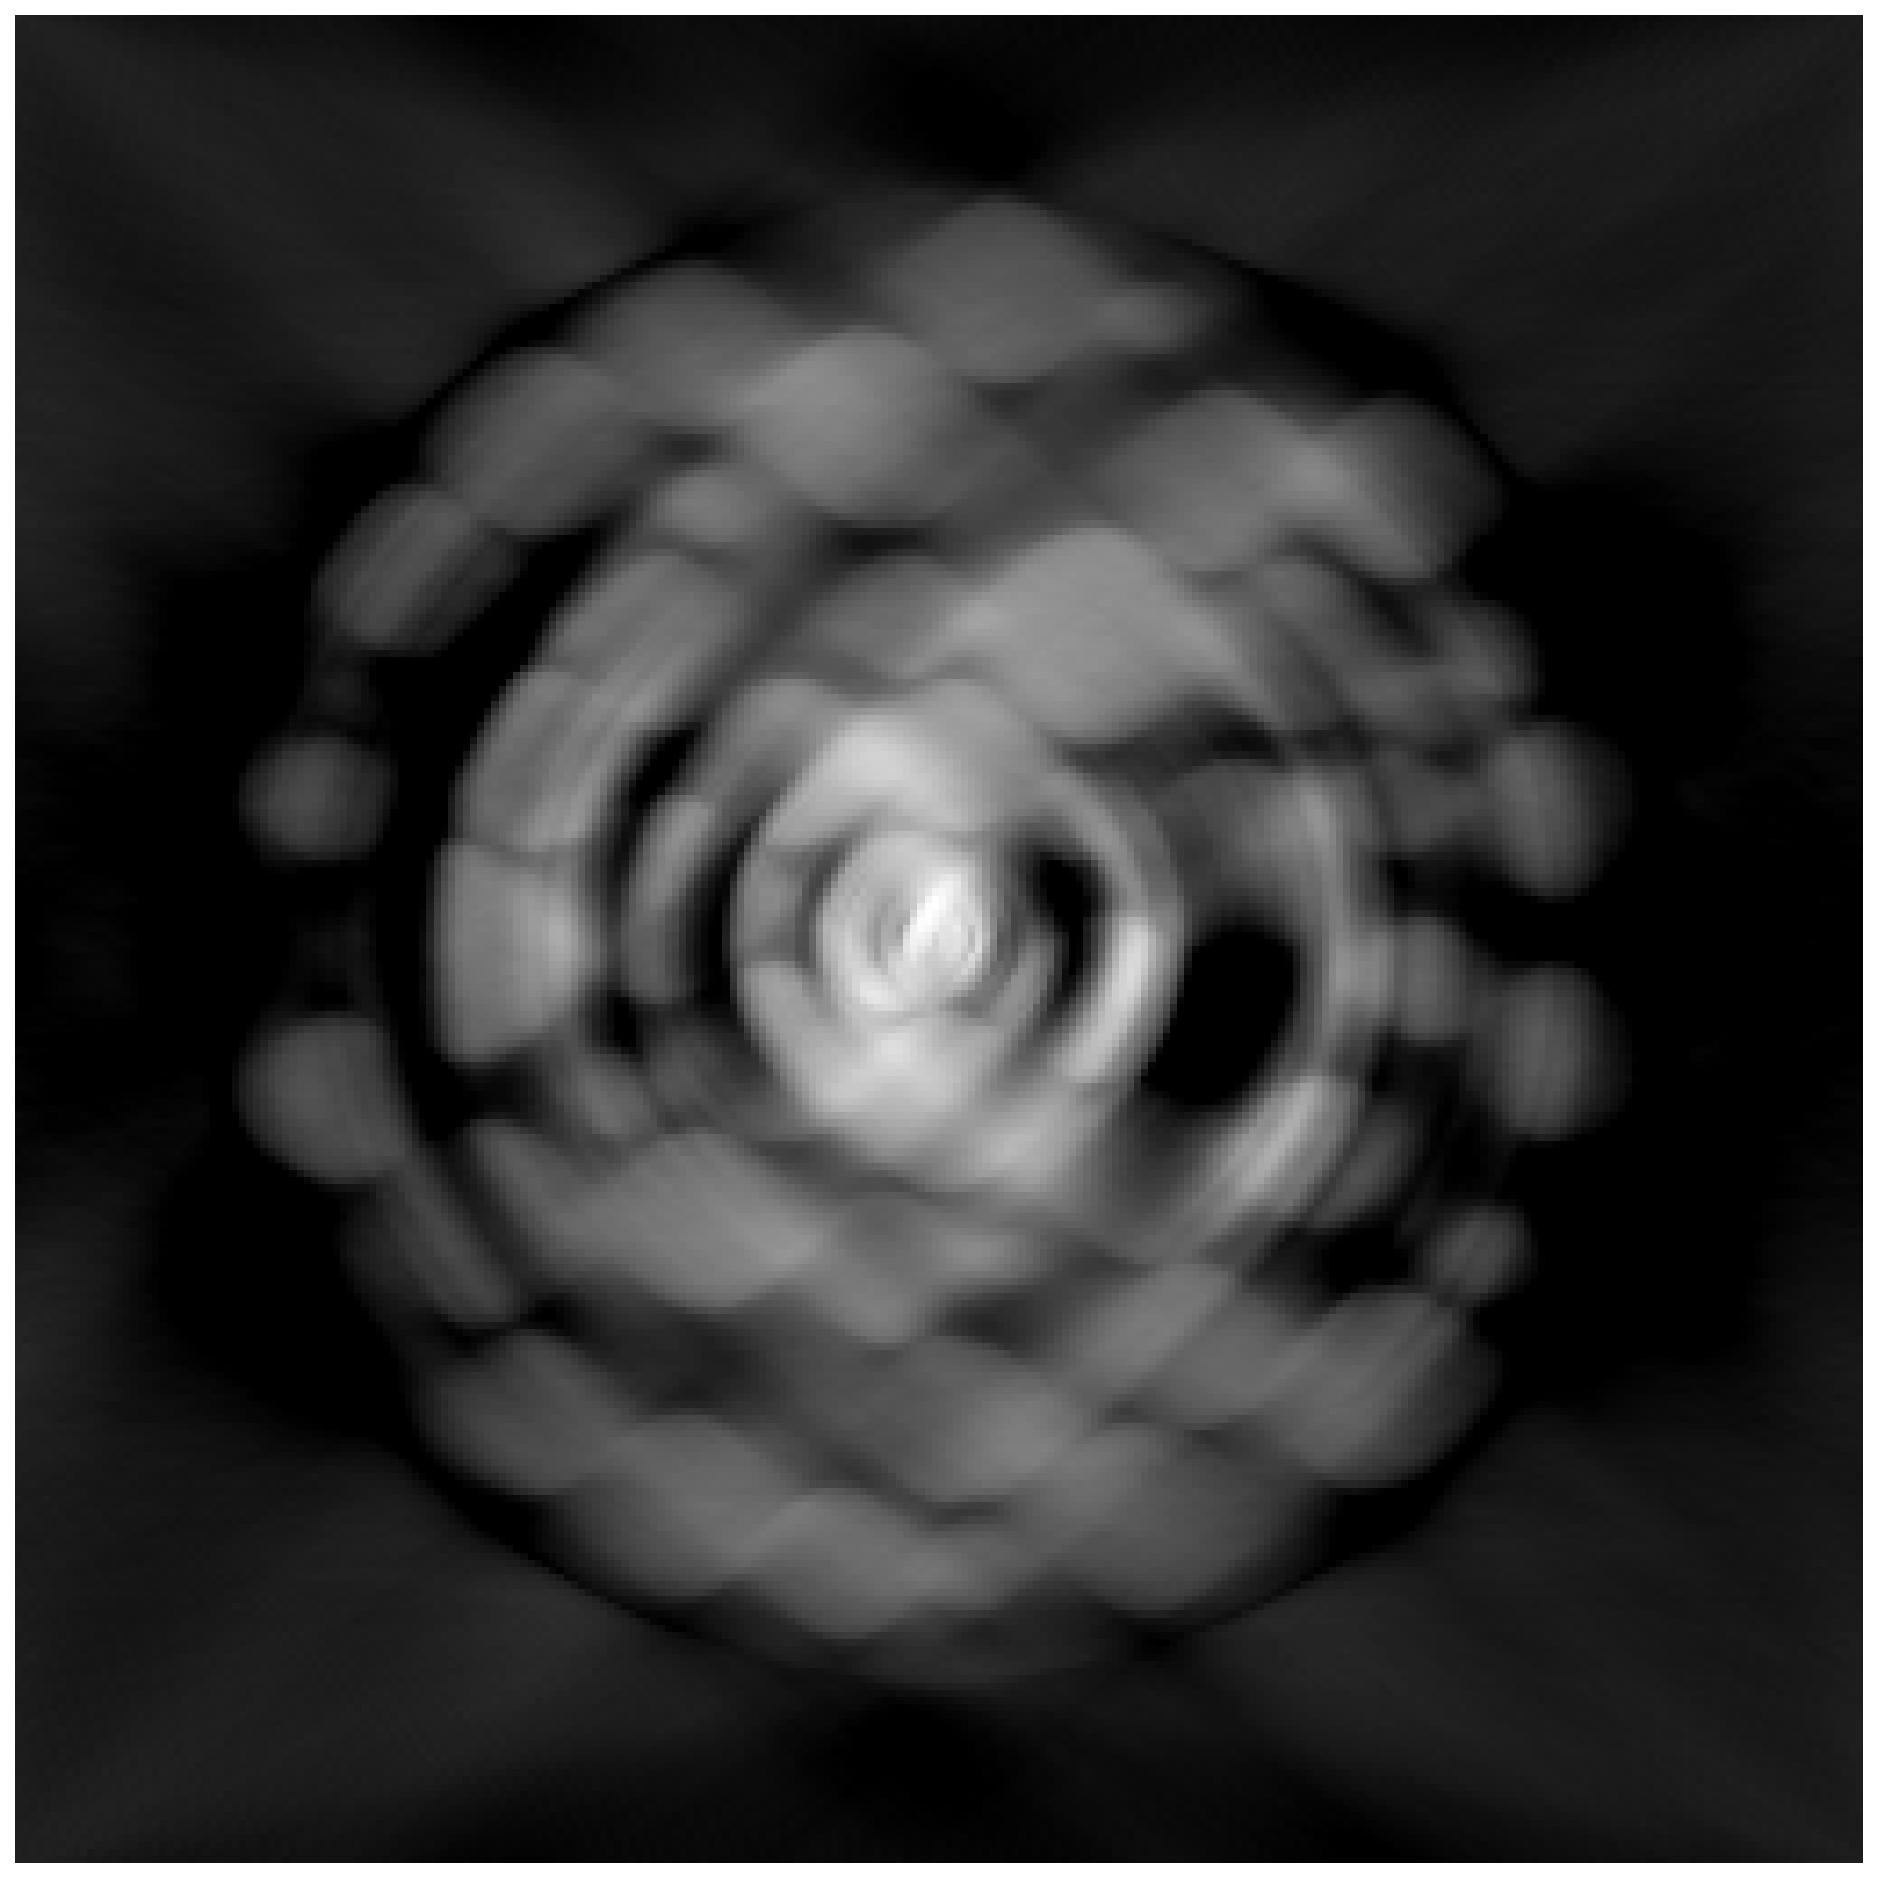
\includegraphics[width=0.2\textwidth]{graphics/reconstructions128_linearInterpolation.jpg}
\label{fig:reconstructions128_linearInterpolation}}
\hfill
\subfloat[Reconstruction with missing acquisitions replaced by CAD-expected ones]{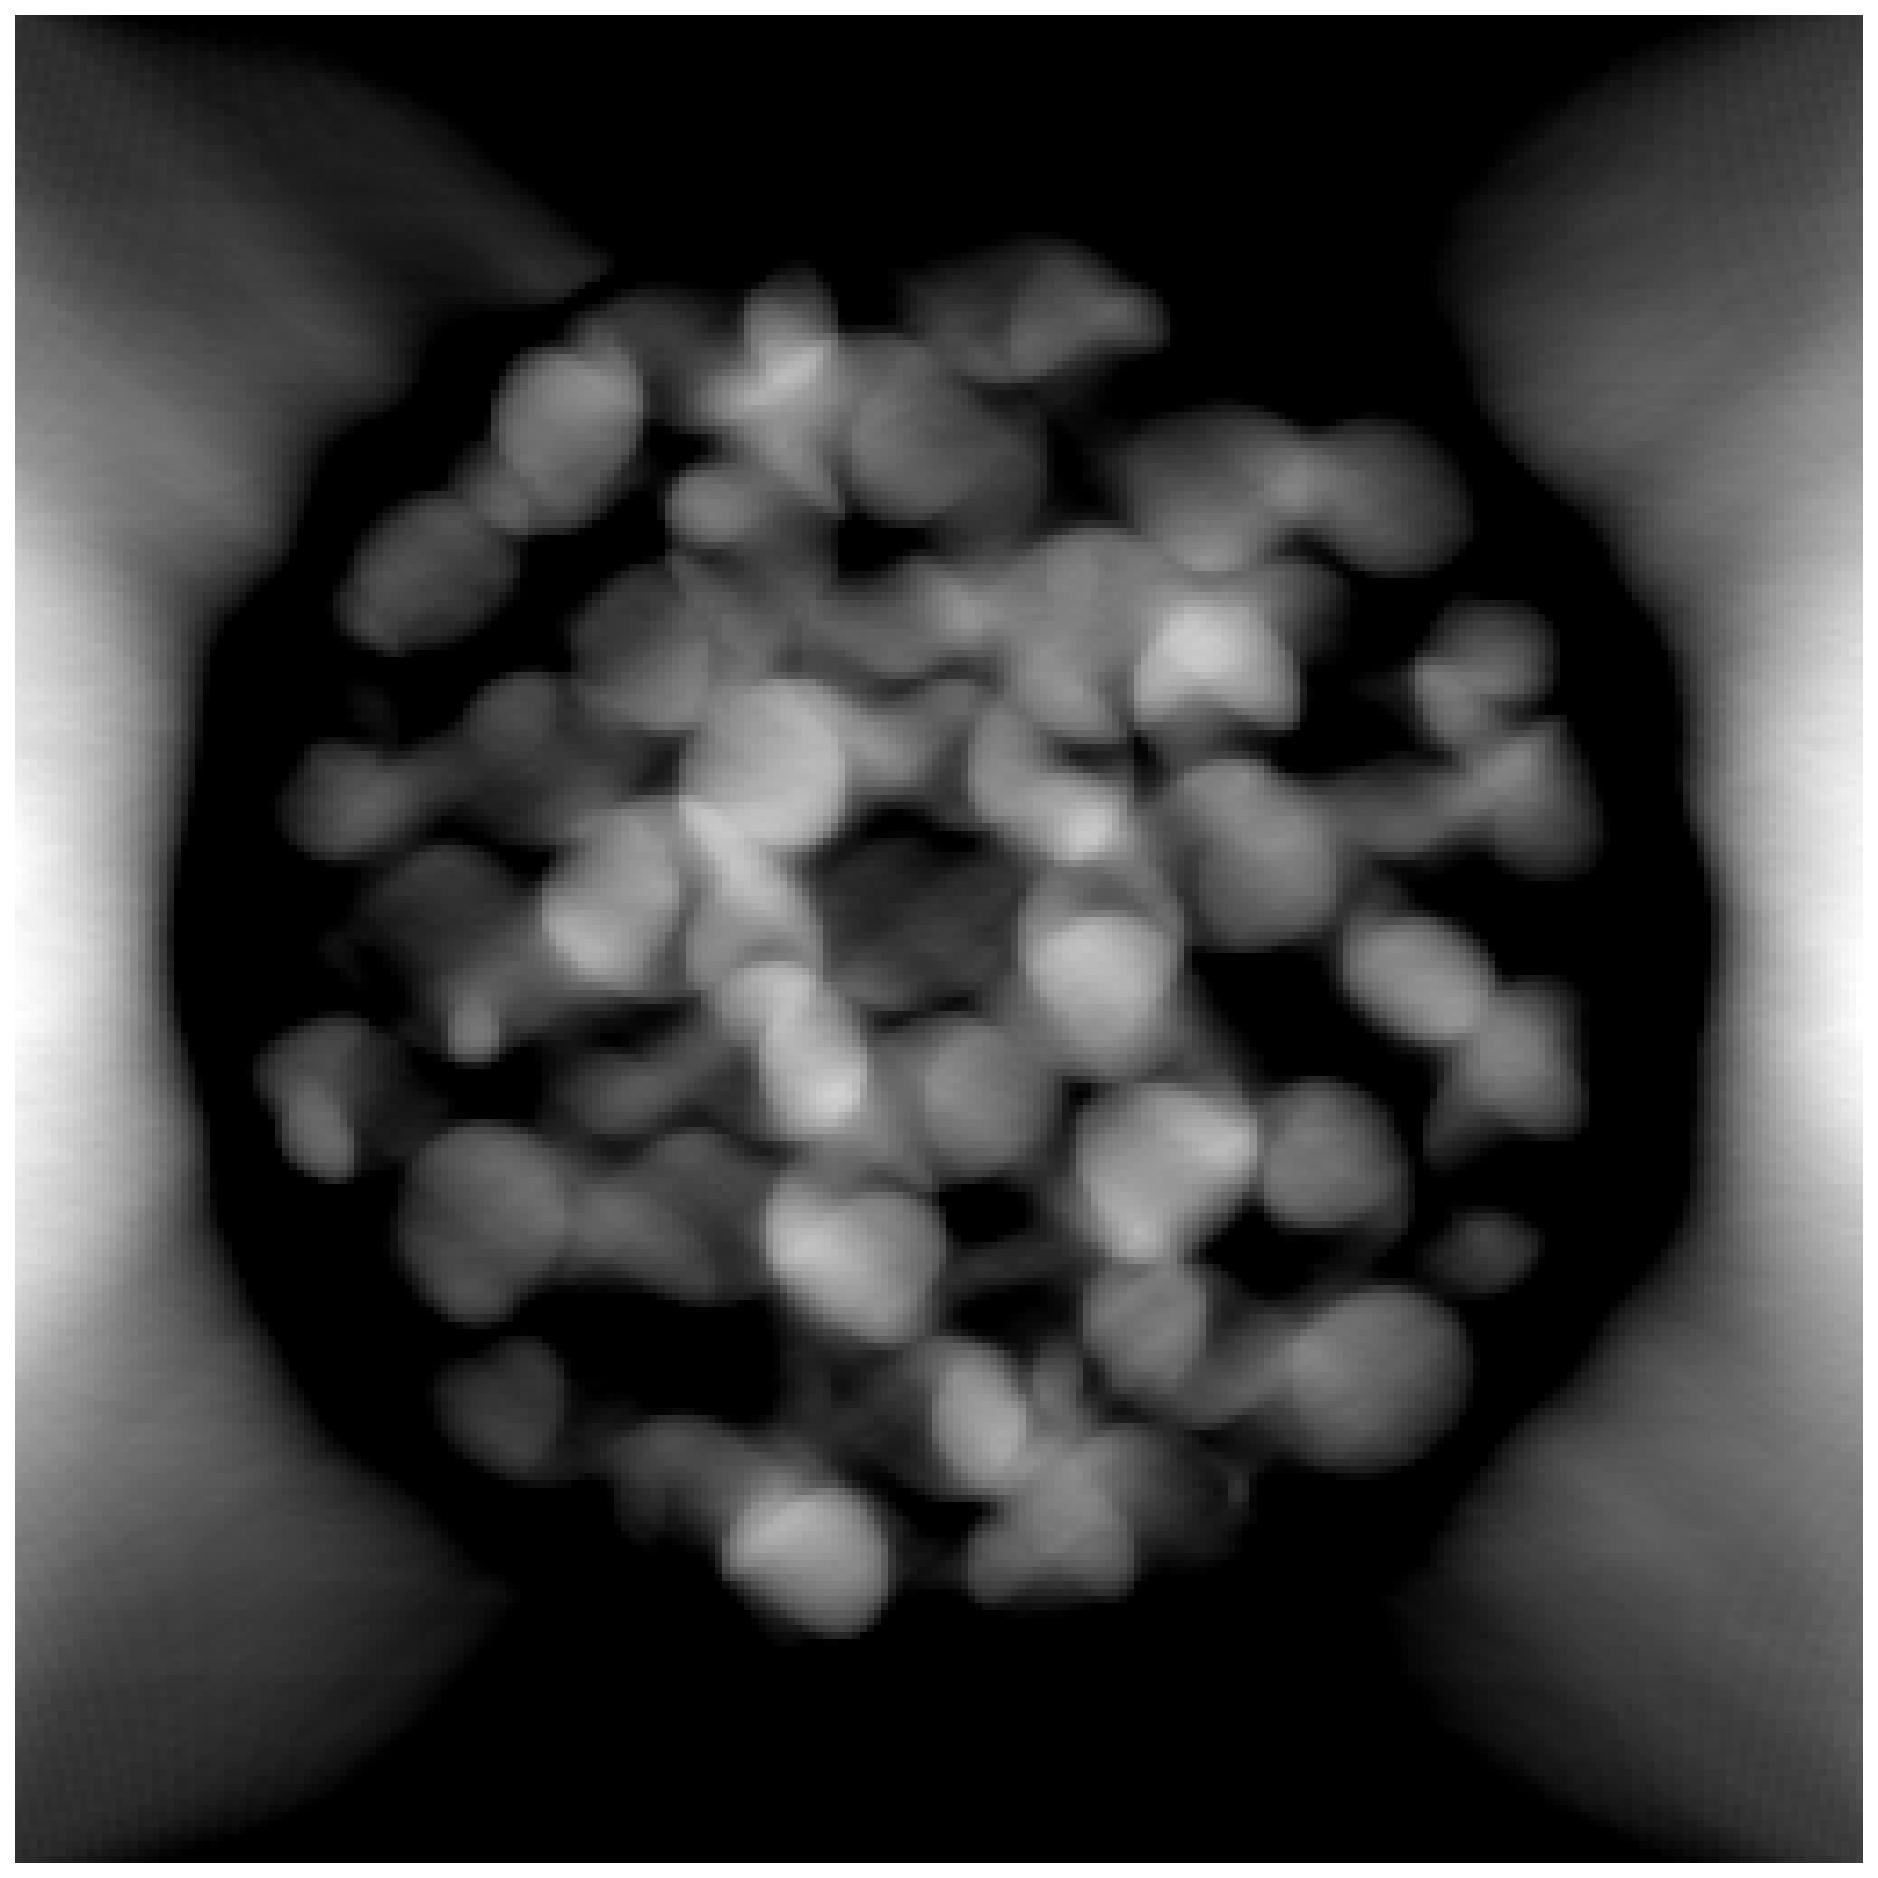
\includegraphics[width=0.2\textwidth]{graphics/reconstructions128_inferenceCad.jpg}
\label{fig:reconstructions128_inferenceCad}}
\hfill
\subfloat[Reconstruction with acquisitions inferred from the Unet without the CAD prior]{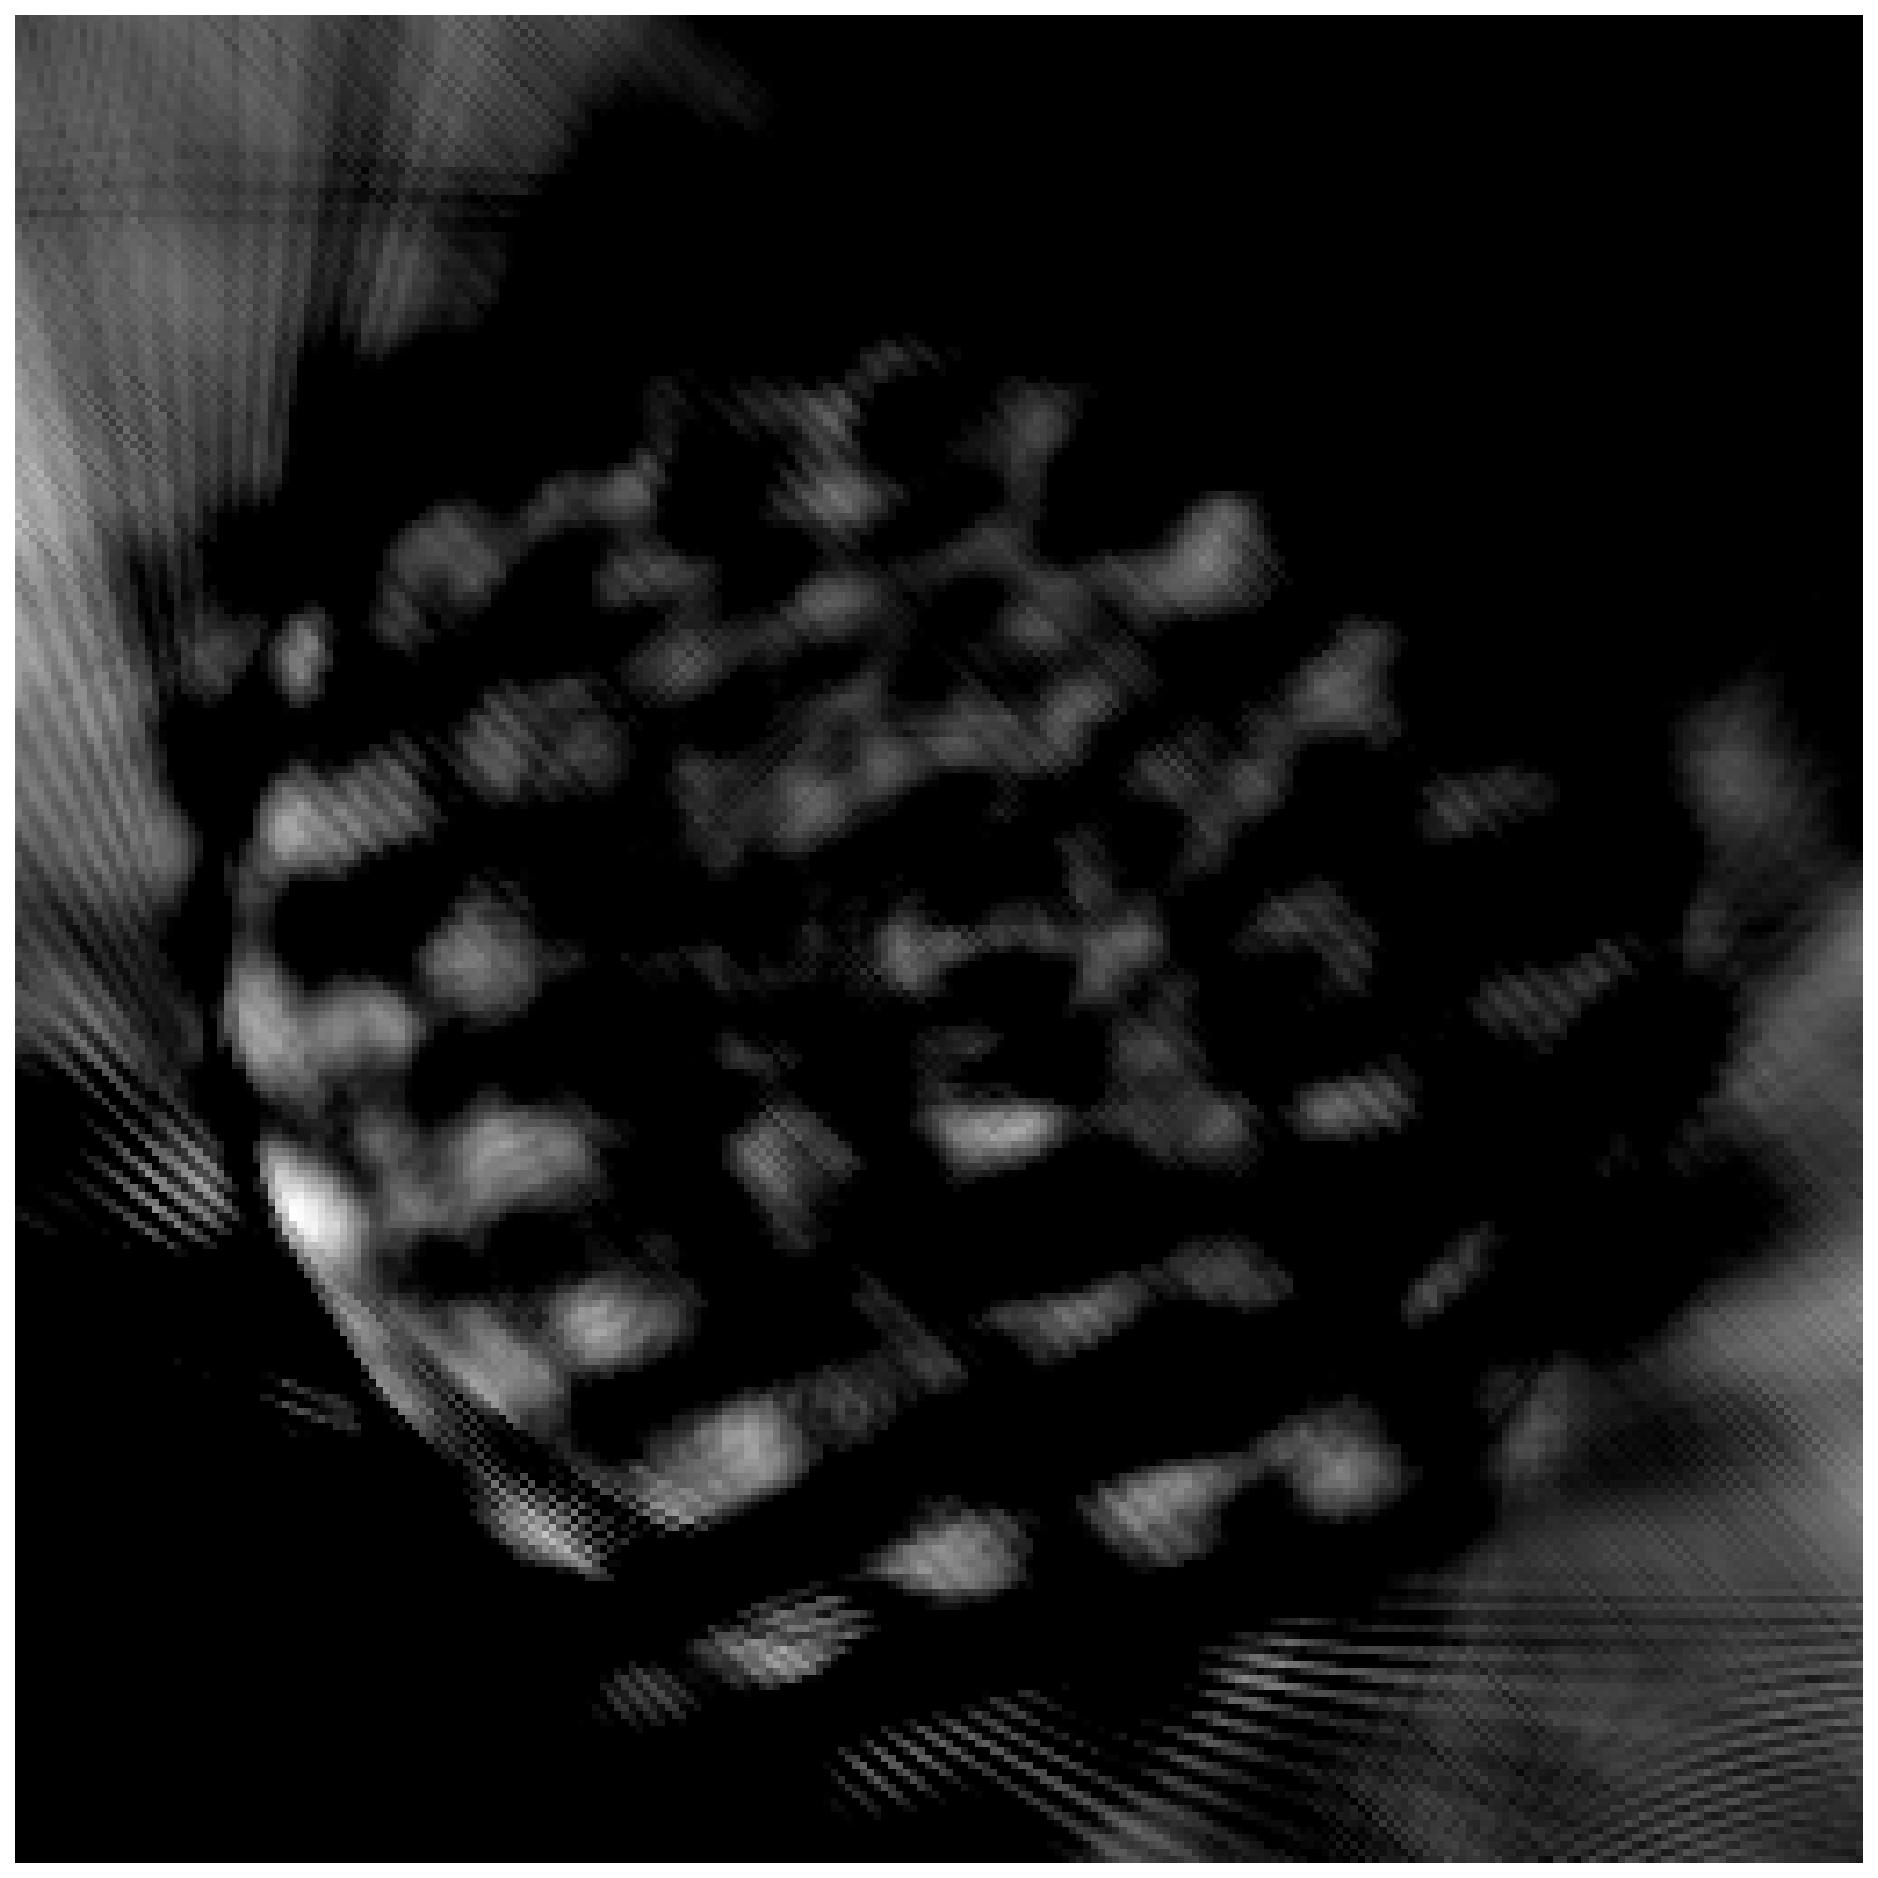
\includegraphics[width=0.2\textwidth]{graphics/reconstructions128_inferenceNoCadUnet.jpg}
\label{fig:reconstructions128_NoCadUnet}}
\hfill
\subfloat[Reconstruction with acquisitions inferred from the Unet with the CAD prior]{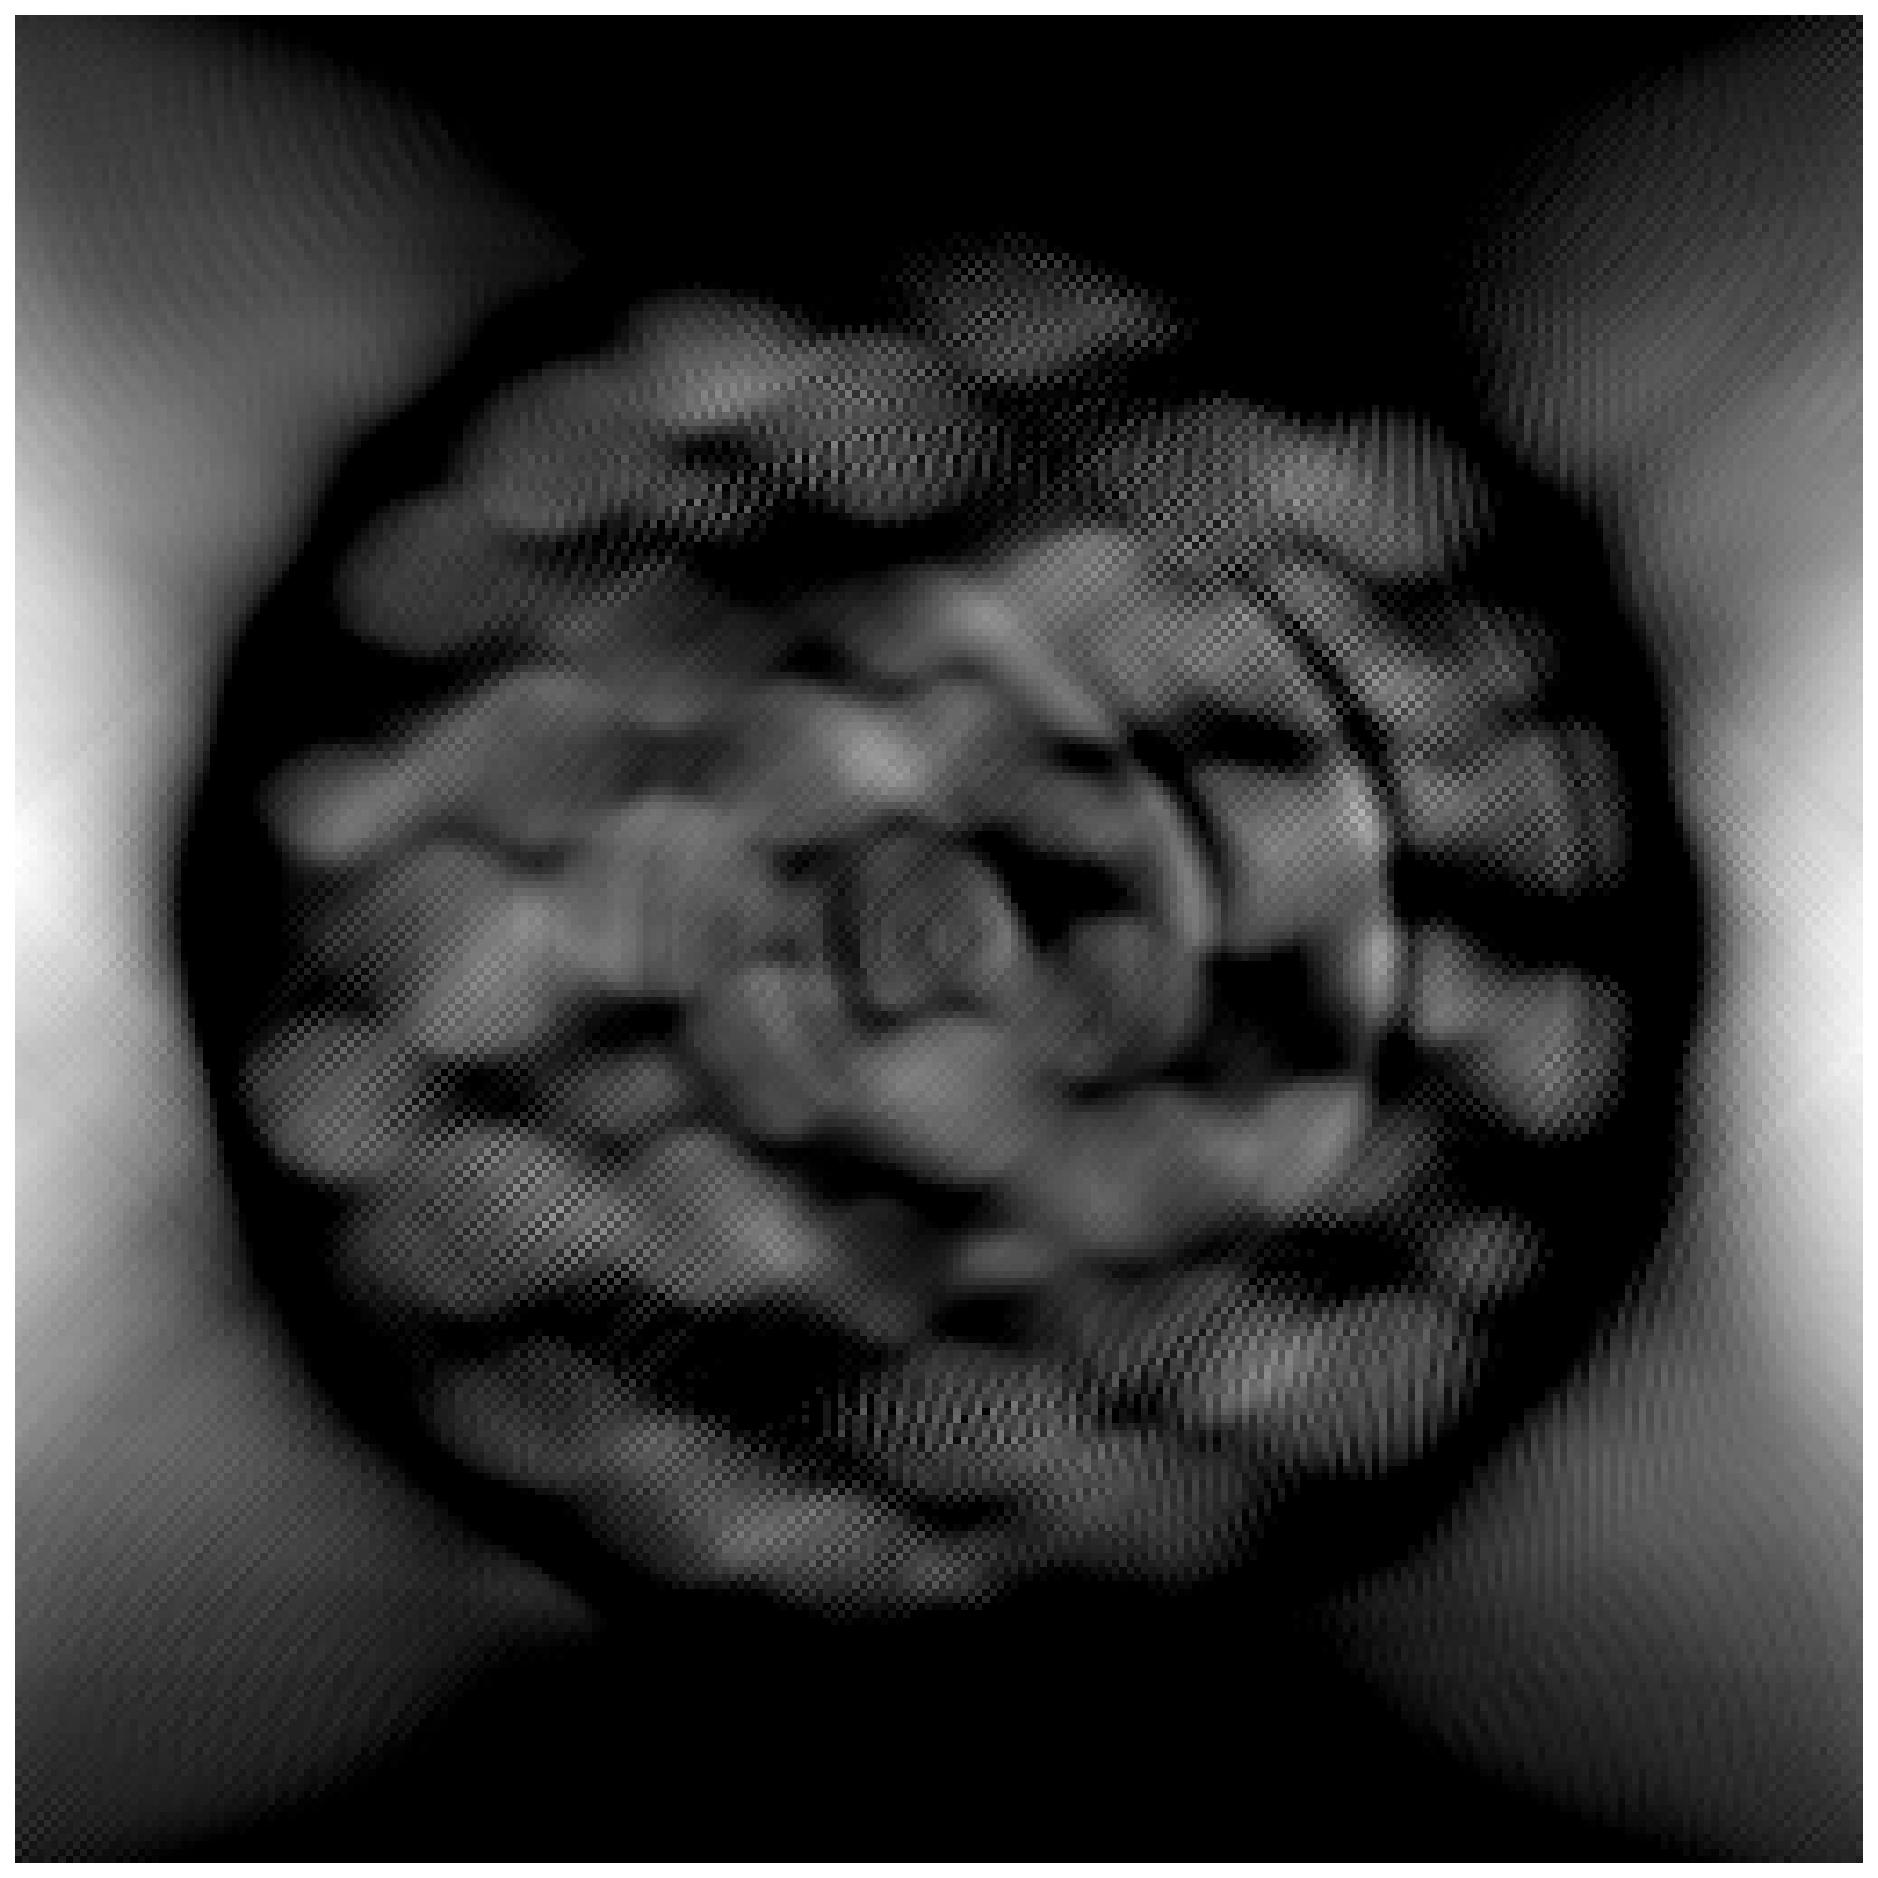
\includegraphics[width=0.2\textwidth]{graphics/reconstructions128_inferenceCadUnet.jpg}
\label{fig:reconstructions128_CadUnet}}
\hfill
\subfloat[Reconstruction with sinogram inpainted by the GAN.]{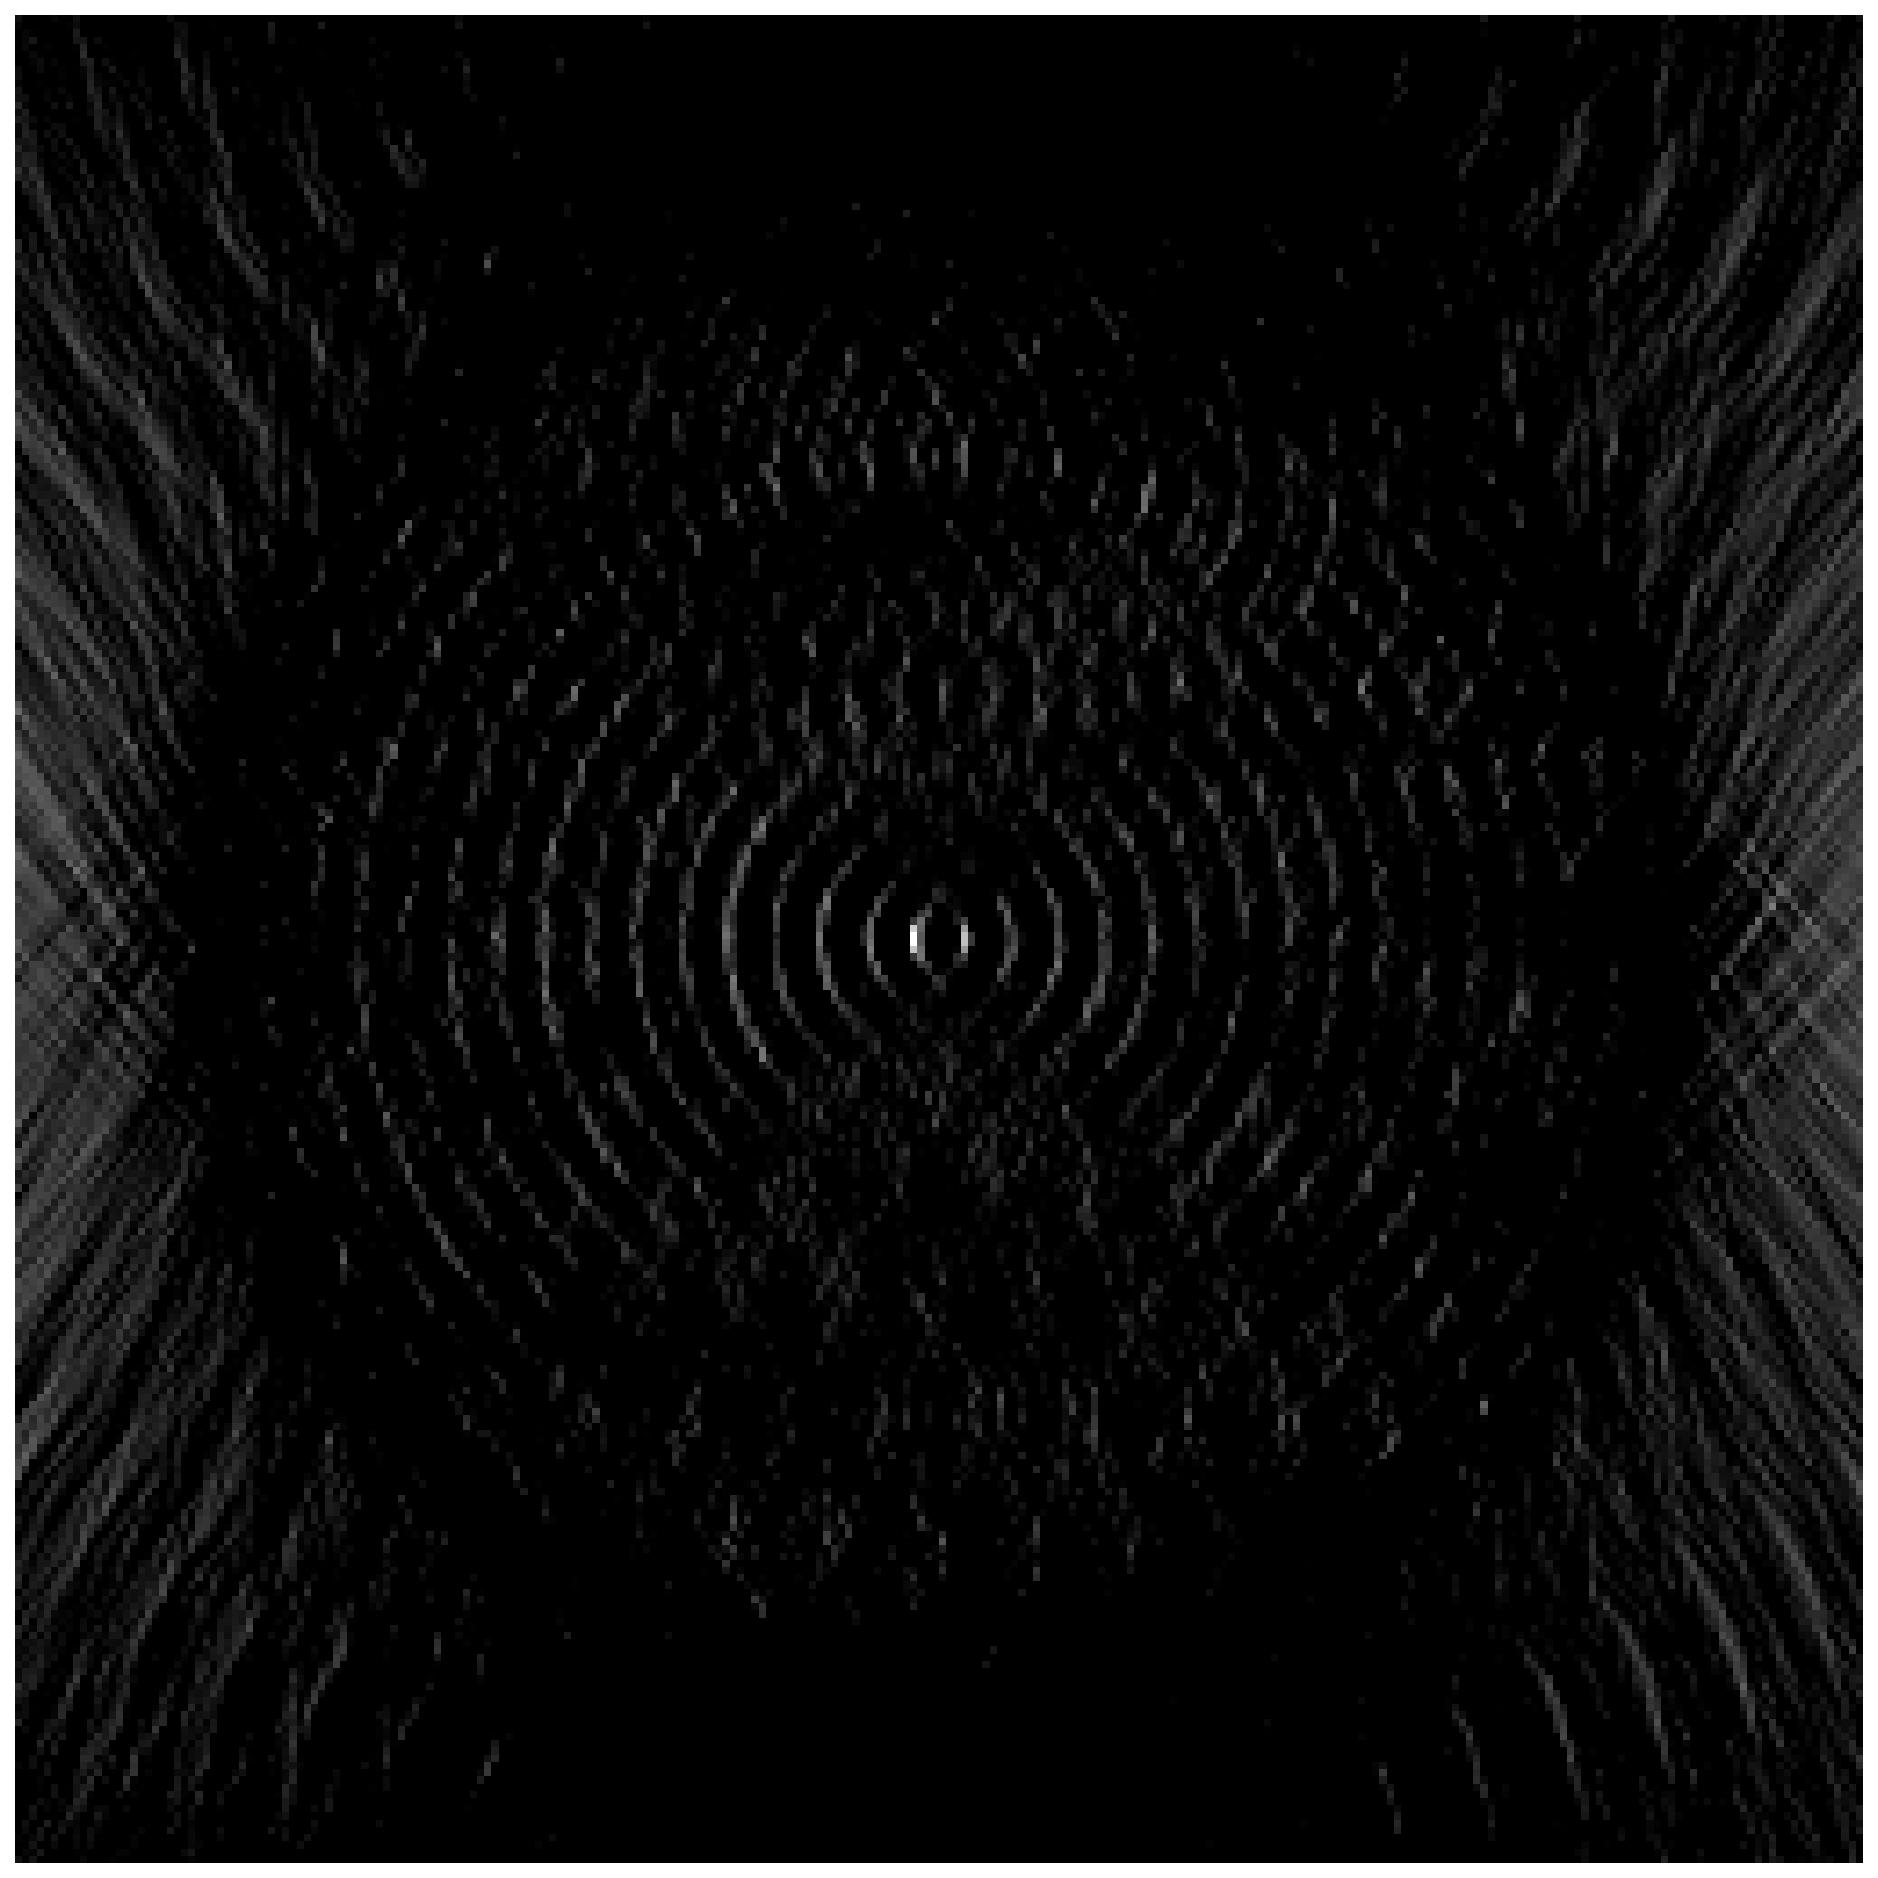
\includegraphics[width=0.2\textwidth]{graphics/reconstructions128_inpaintingNoCadGan.jpg}
\label{fig:reconstructions128_NoCadGan}}
\hfill
\subfloat[Reconstruction with missing acquisitions inferred from the pix2pix architecture using CAD prior.]{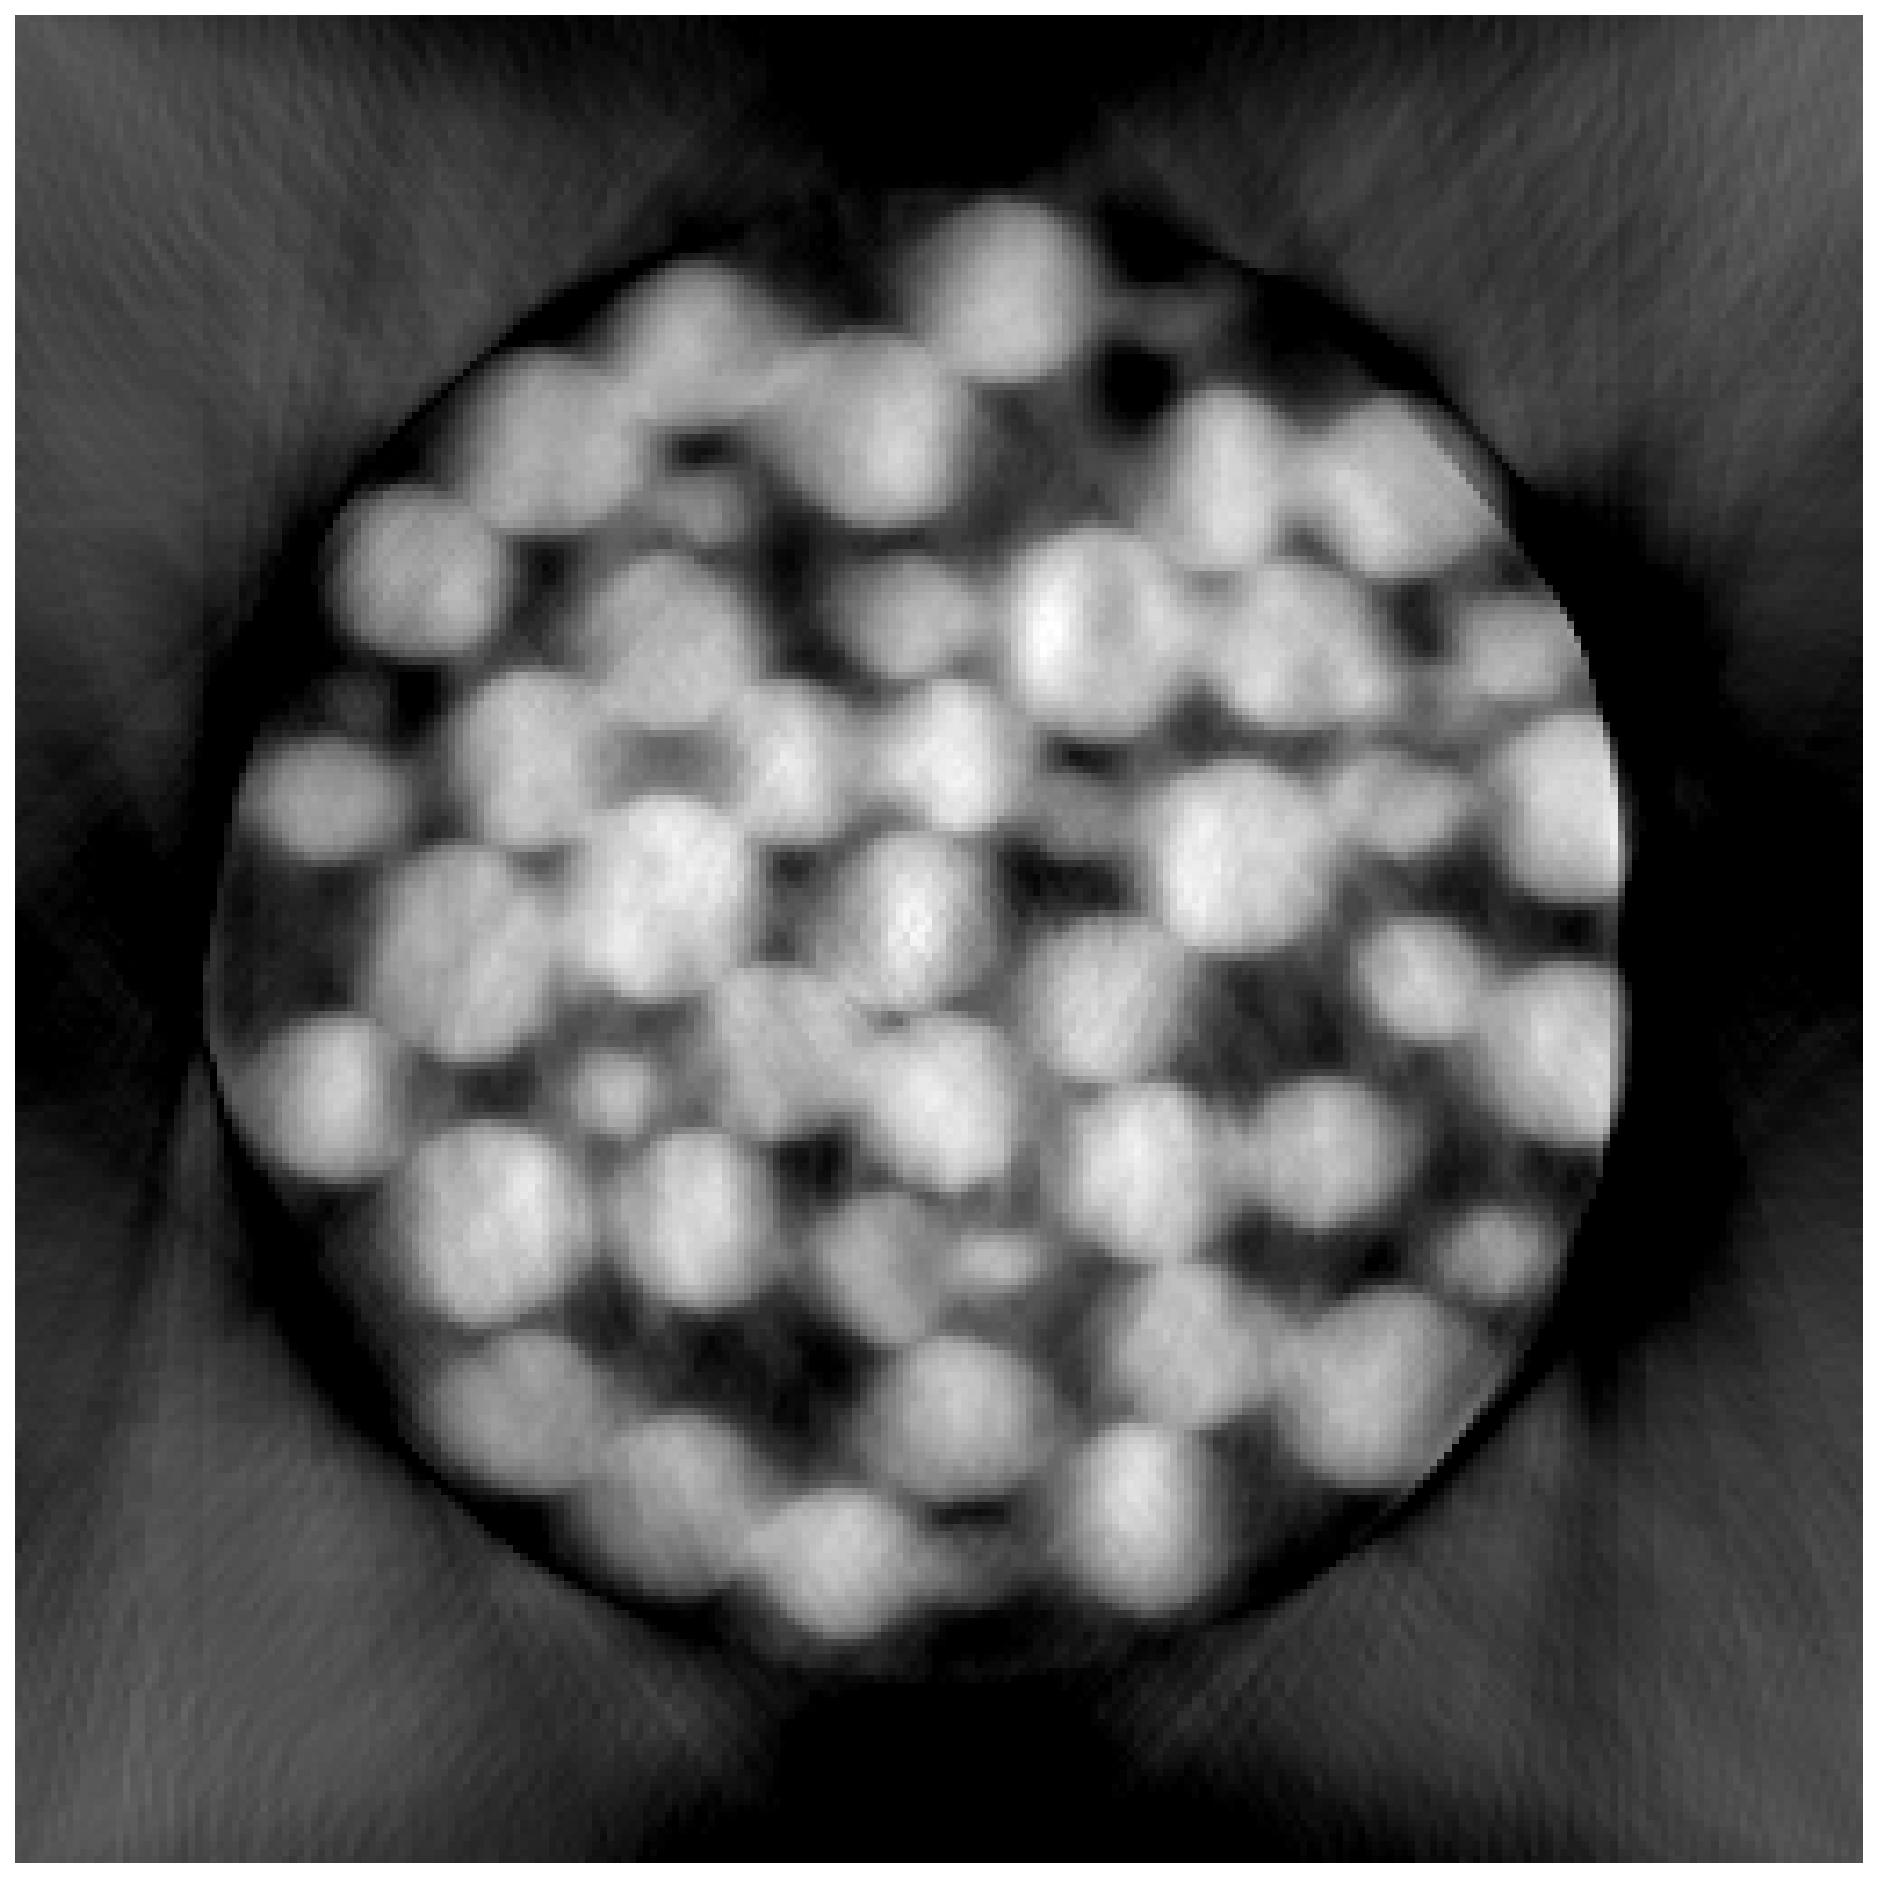
\includegraphics[width=0.2\textwidth]{graphics/reconstructions128_inferenceCadGan.jpg}
\label{fig:reconstructions128_CadGan}}

\label{fig:reconstructions}
\caption{Reconstructions of the first sample of the SophiaBeads test dataset.(\ref{fig:reconstructions128_target}) is the target image, reconstructed from all 256 acquisitions and (\ref{fig:reconstructions128_noInterpolation}) is the image reconstructed from the scarce sinogram. (\ref{fig:reconstructions128_linearInterpolation}) to (\ref{fig:reconstructions128_CadGan}) are the images reconstructed from sinograms enhanced with various methods.}
\end{figure*}  

\begin{figure*}
\centering
\subfloat[Target reconstruction.]{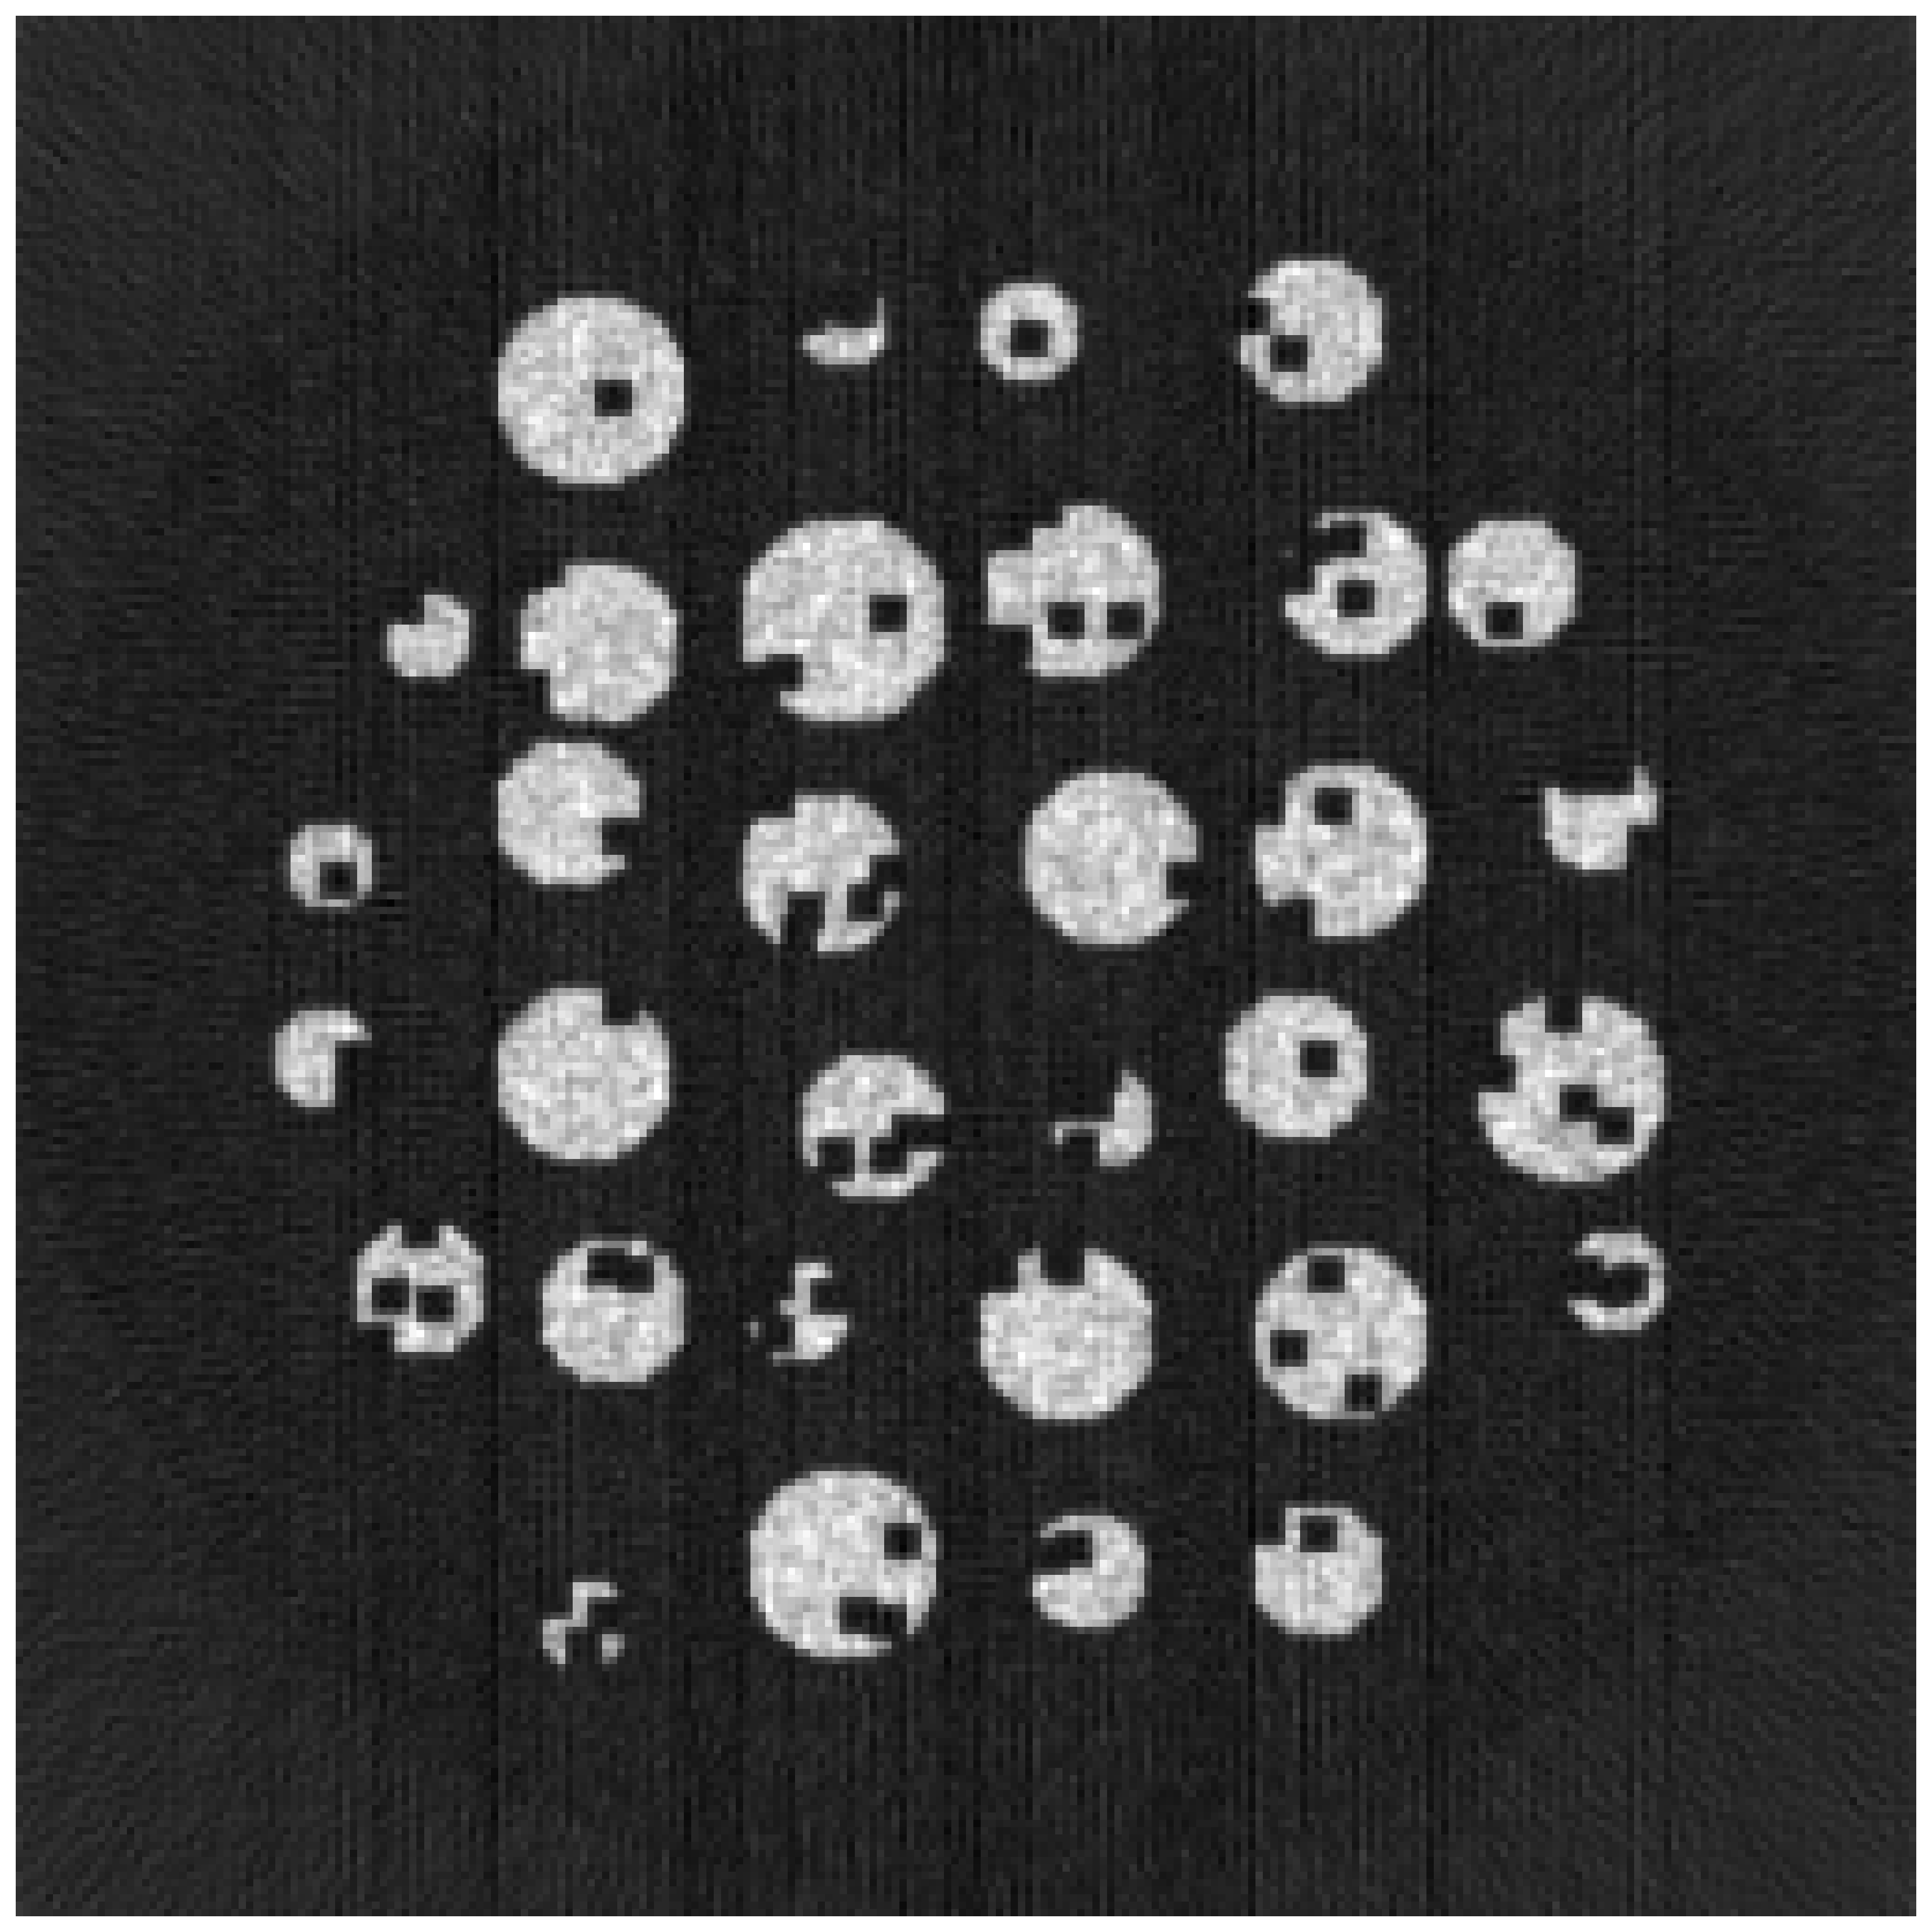
\includegraphics[width=0.15\textwidth]{graphics/holes_tar.png}
\label{fig:holes_tar}}
\hfill
\subfloat[Reconstruction using our method.]{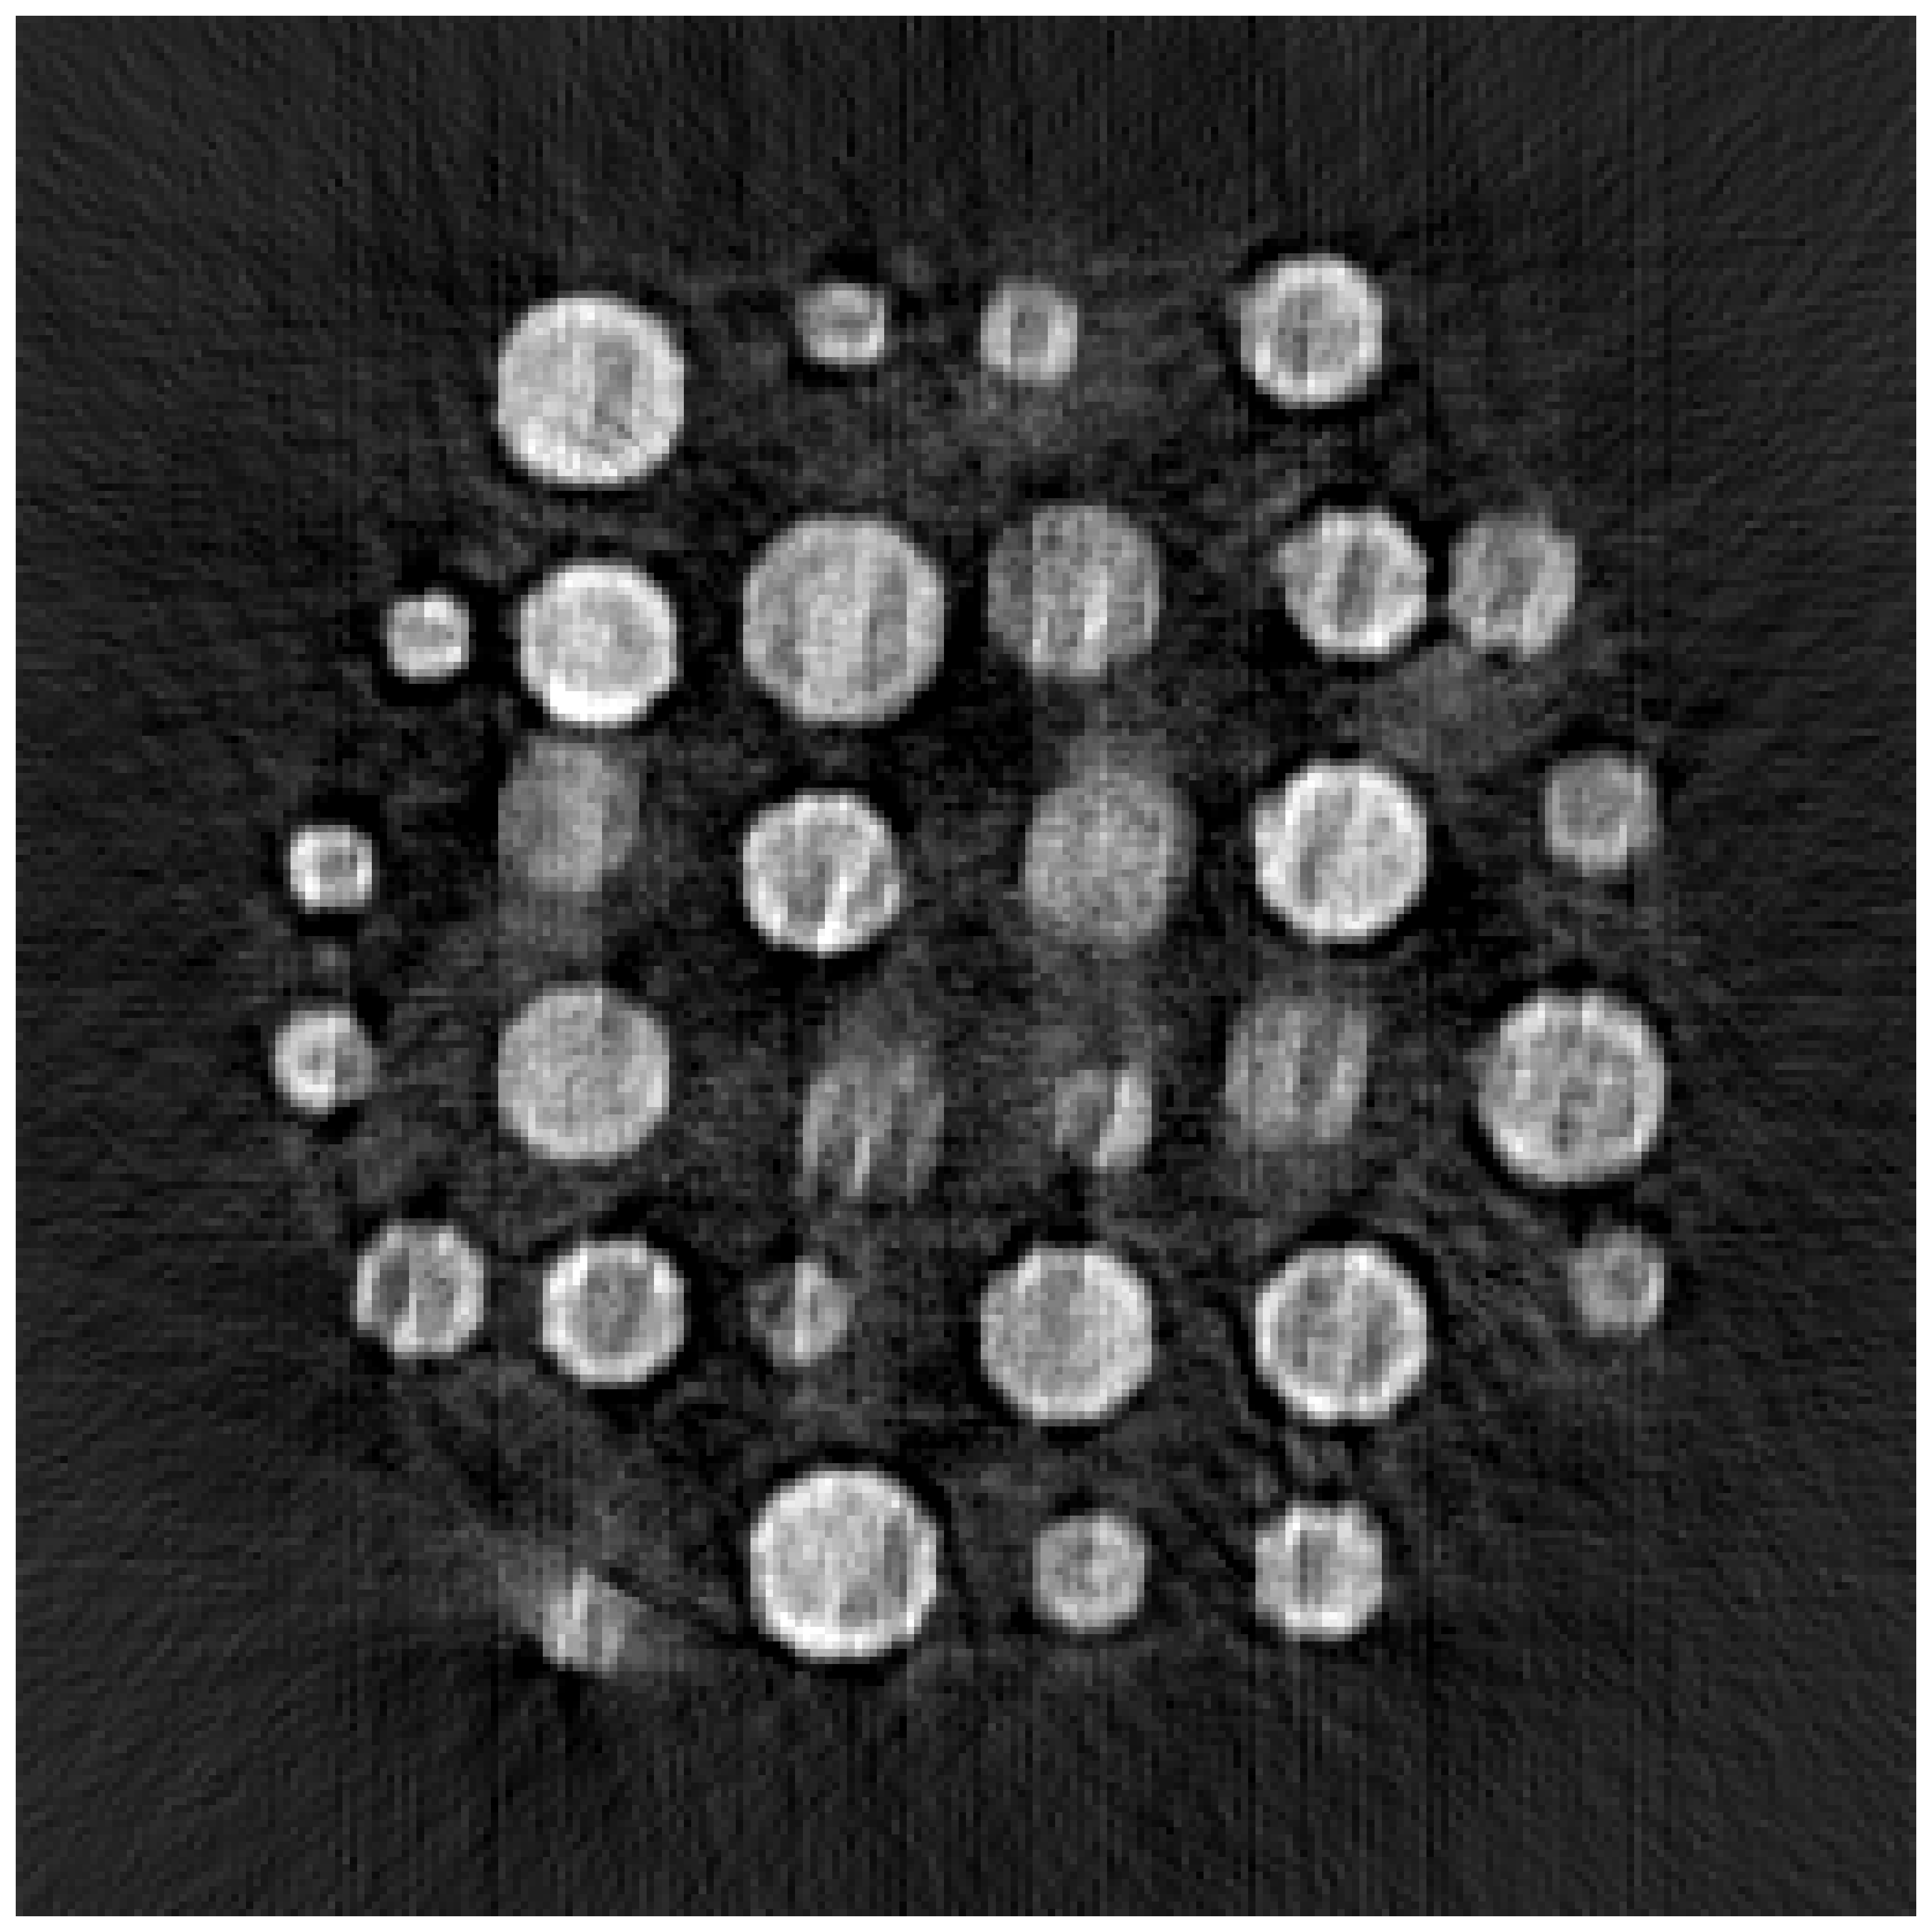
\includegraphics[width=0.15\textwidth]{graphics/holes_gan.png}
\label{fig:holes_gan}}
\hfill
\subfloat[Difference between the image reconstructed with our method and the target reconstruction.]{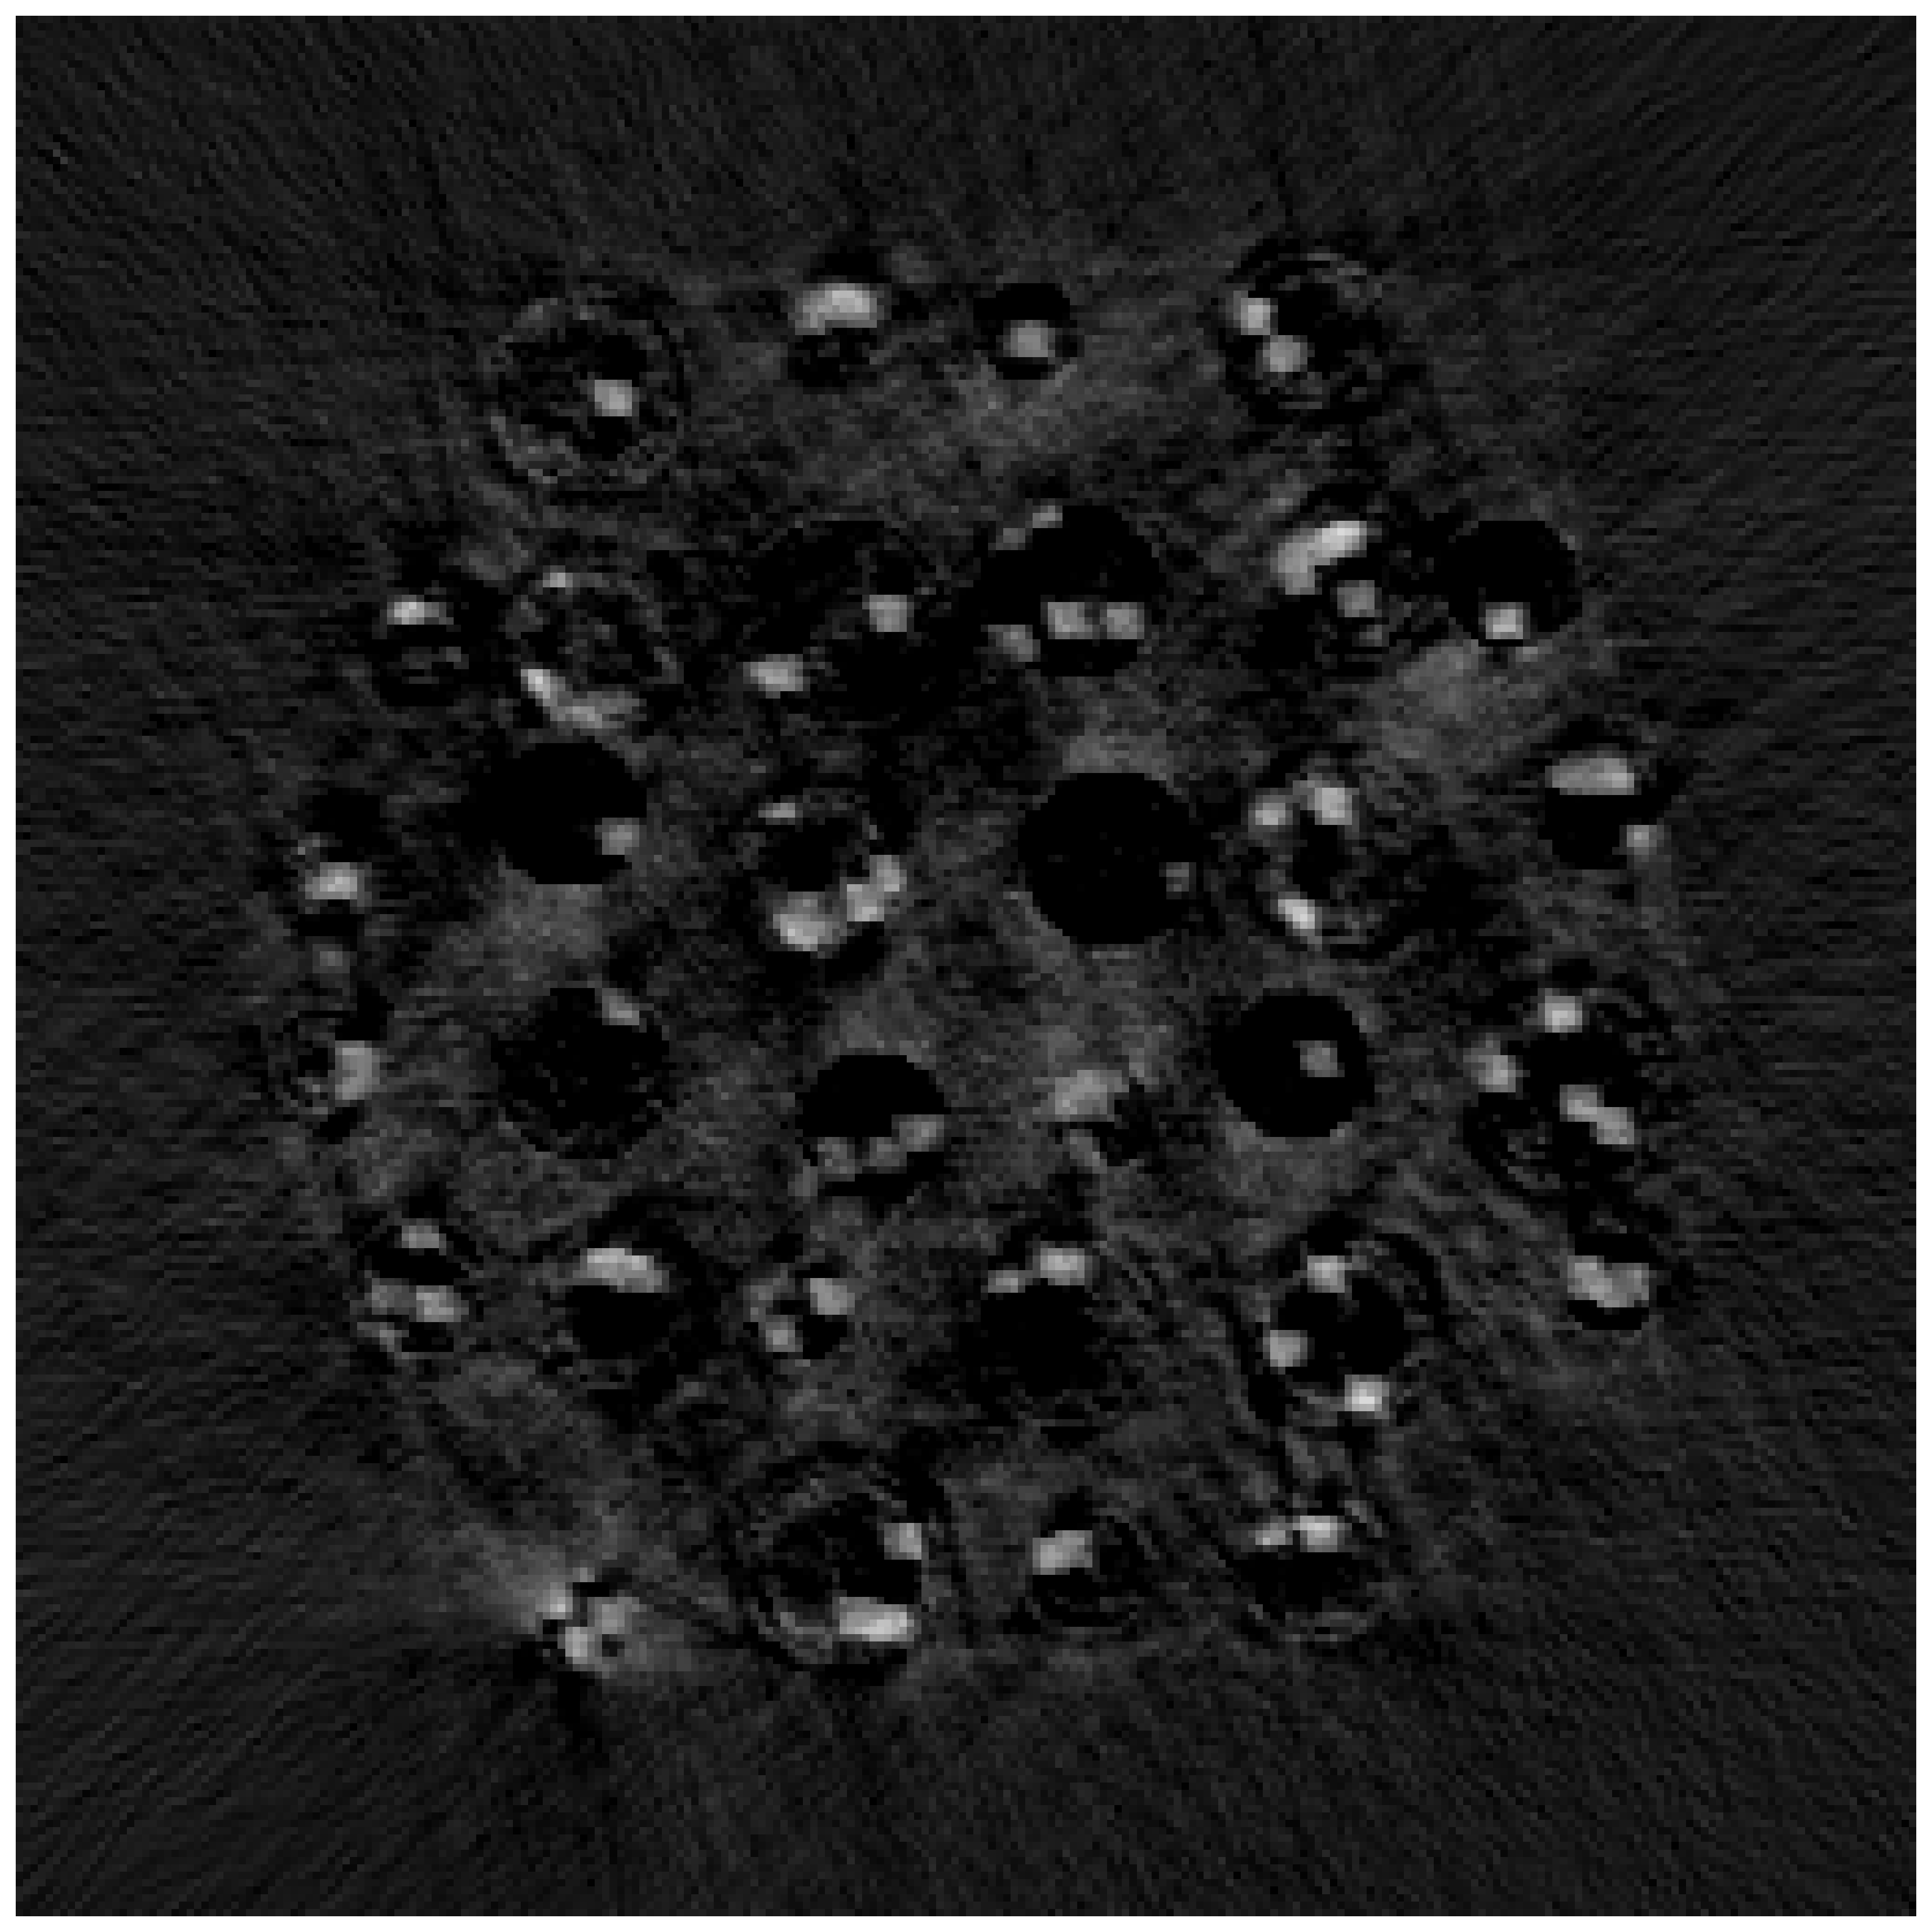
\includegraphics[width=0.15\textwidth]{graphics/holes_gan_tar.png}
\label{fig:holes_gan_tar}}
\hfill
\subfloat[Reconstruction using the shape prior.]{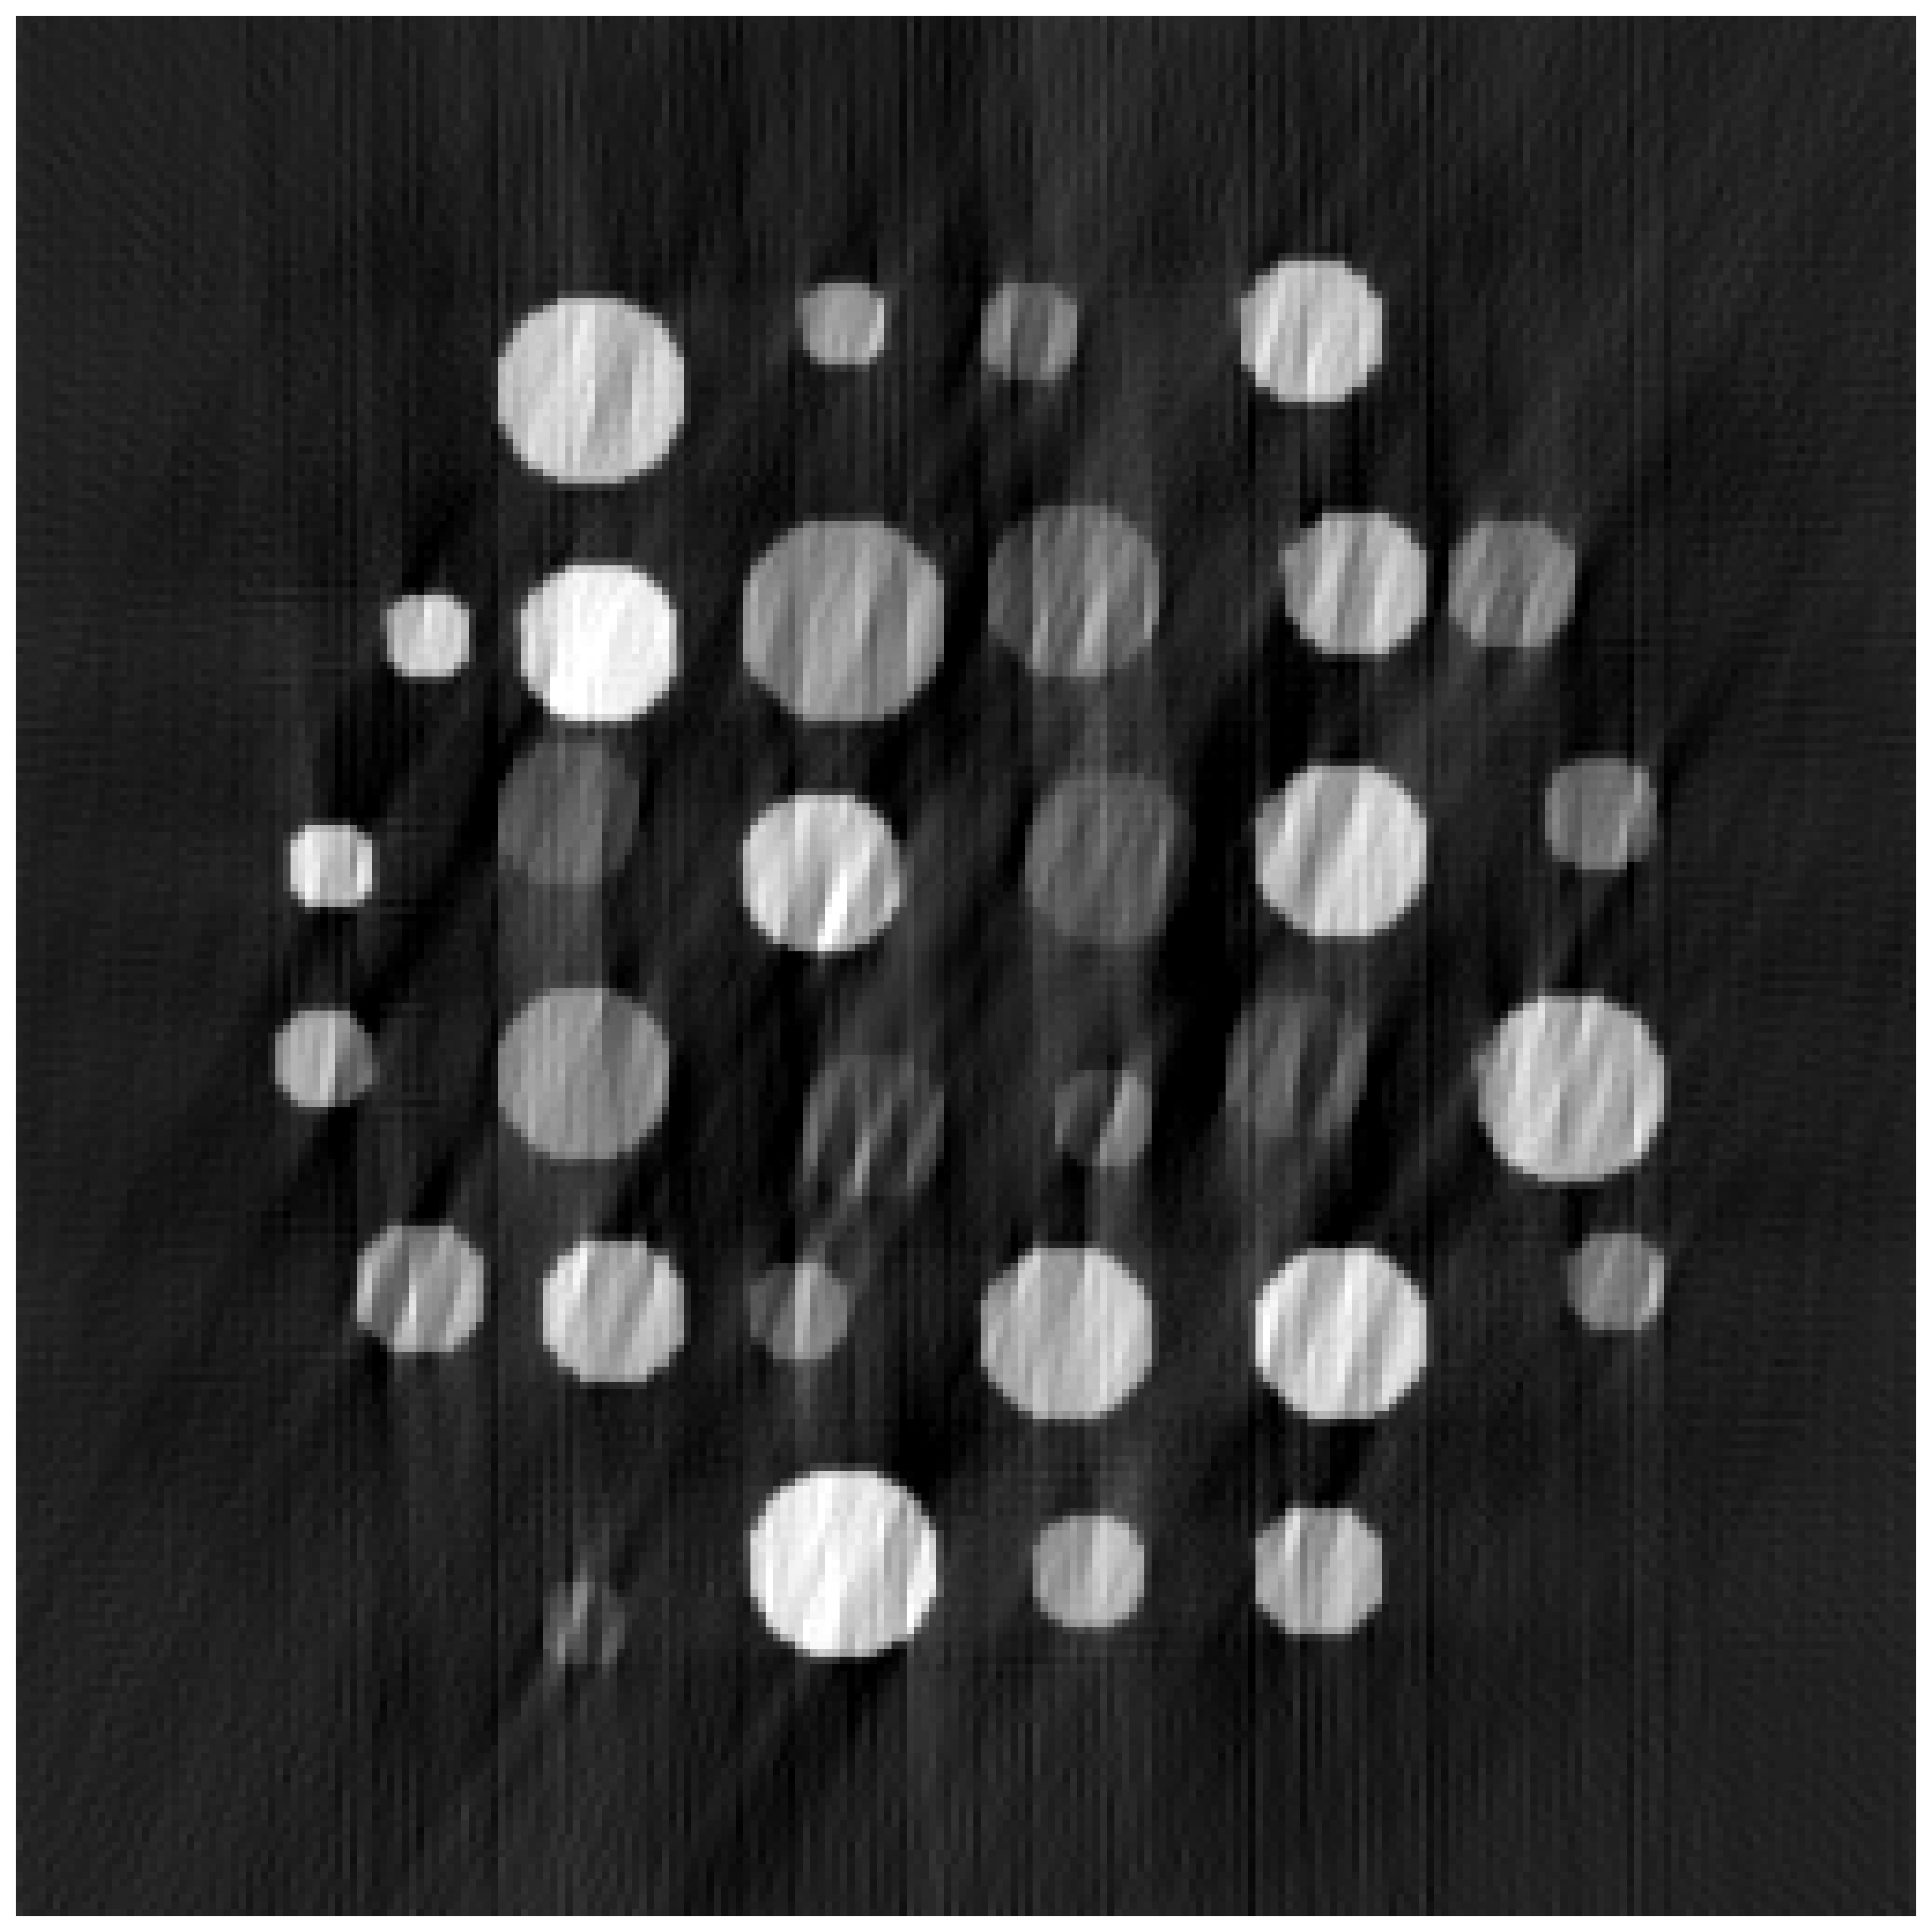
\includegraphics[width=0.15\textwidth]{graphics/holes_cad.png}
\label{fig:holes_cad}}
\hfill
\subfloat[Difference between the image reconstructed with the shape prior and the target reconstruction.]{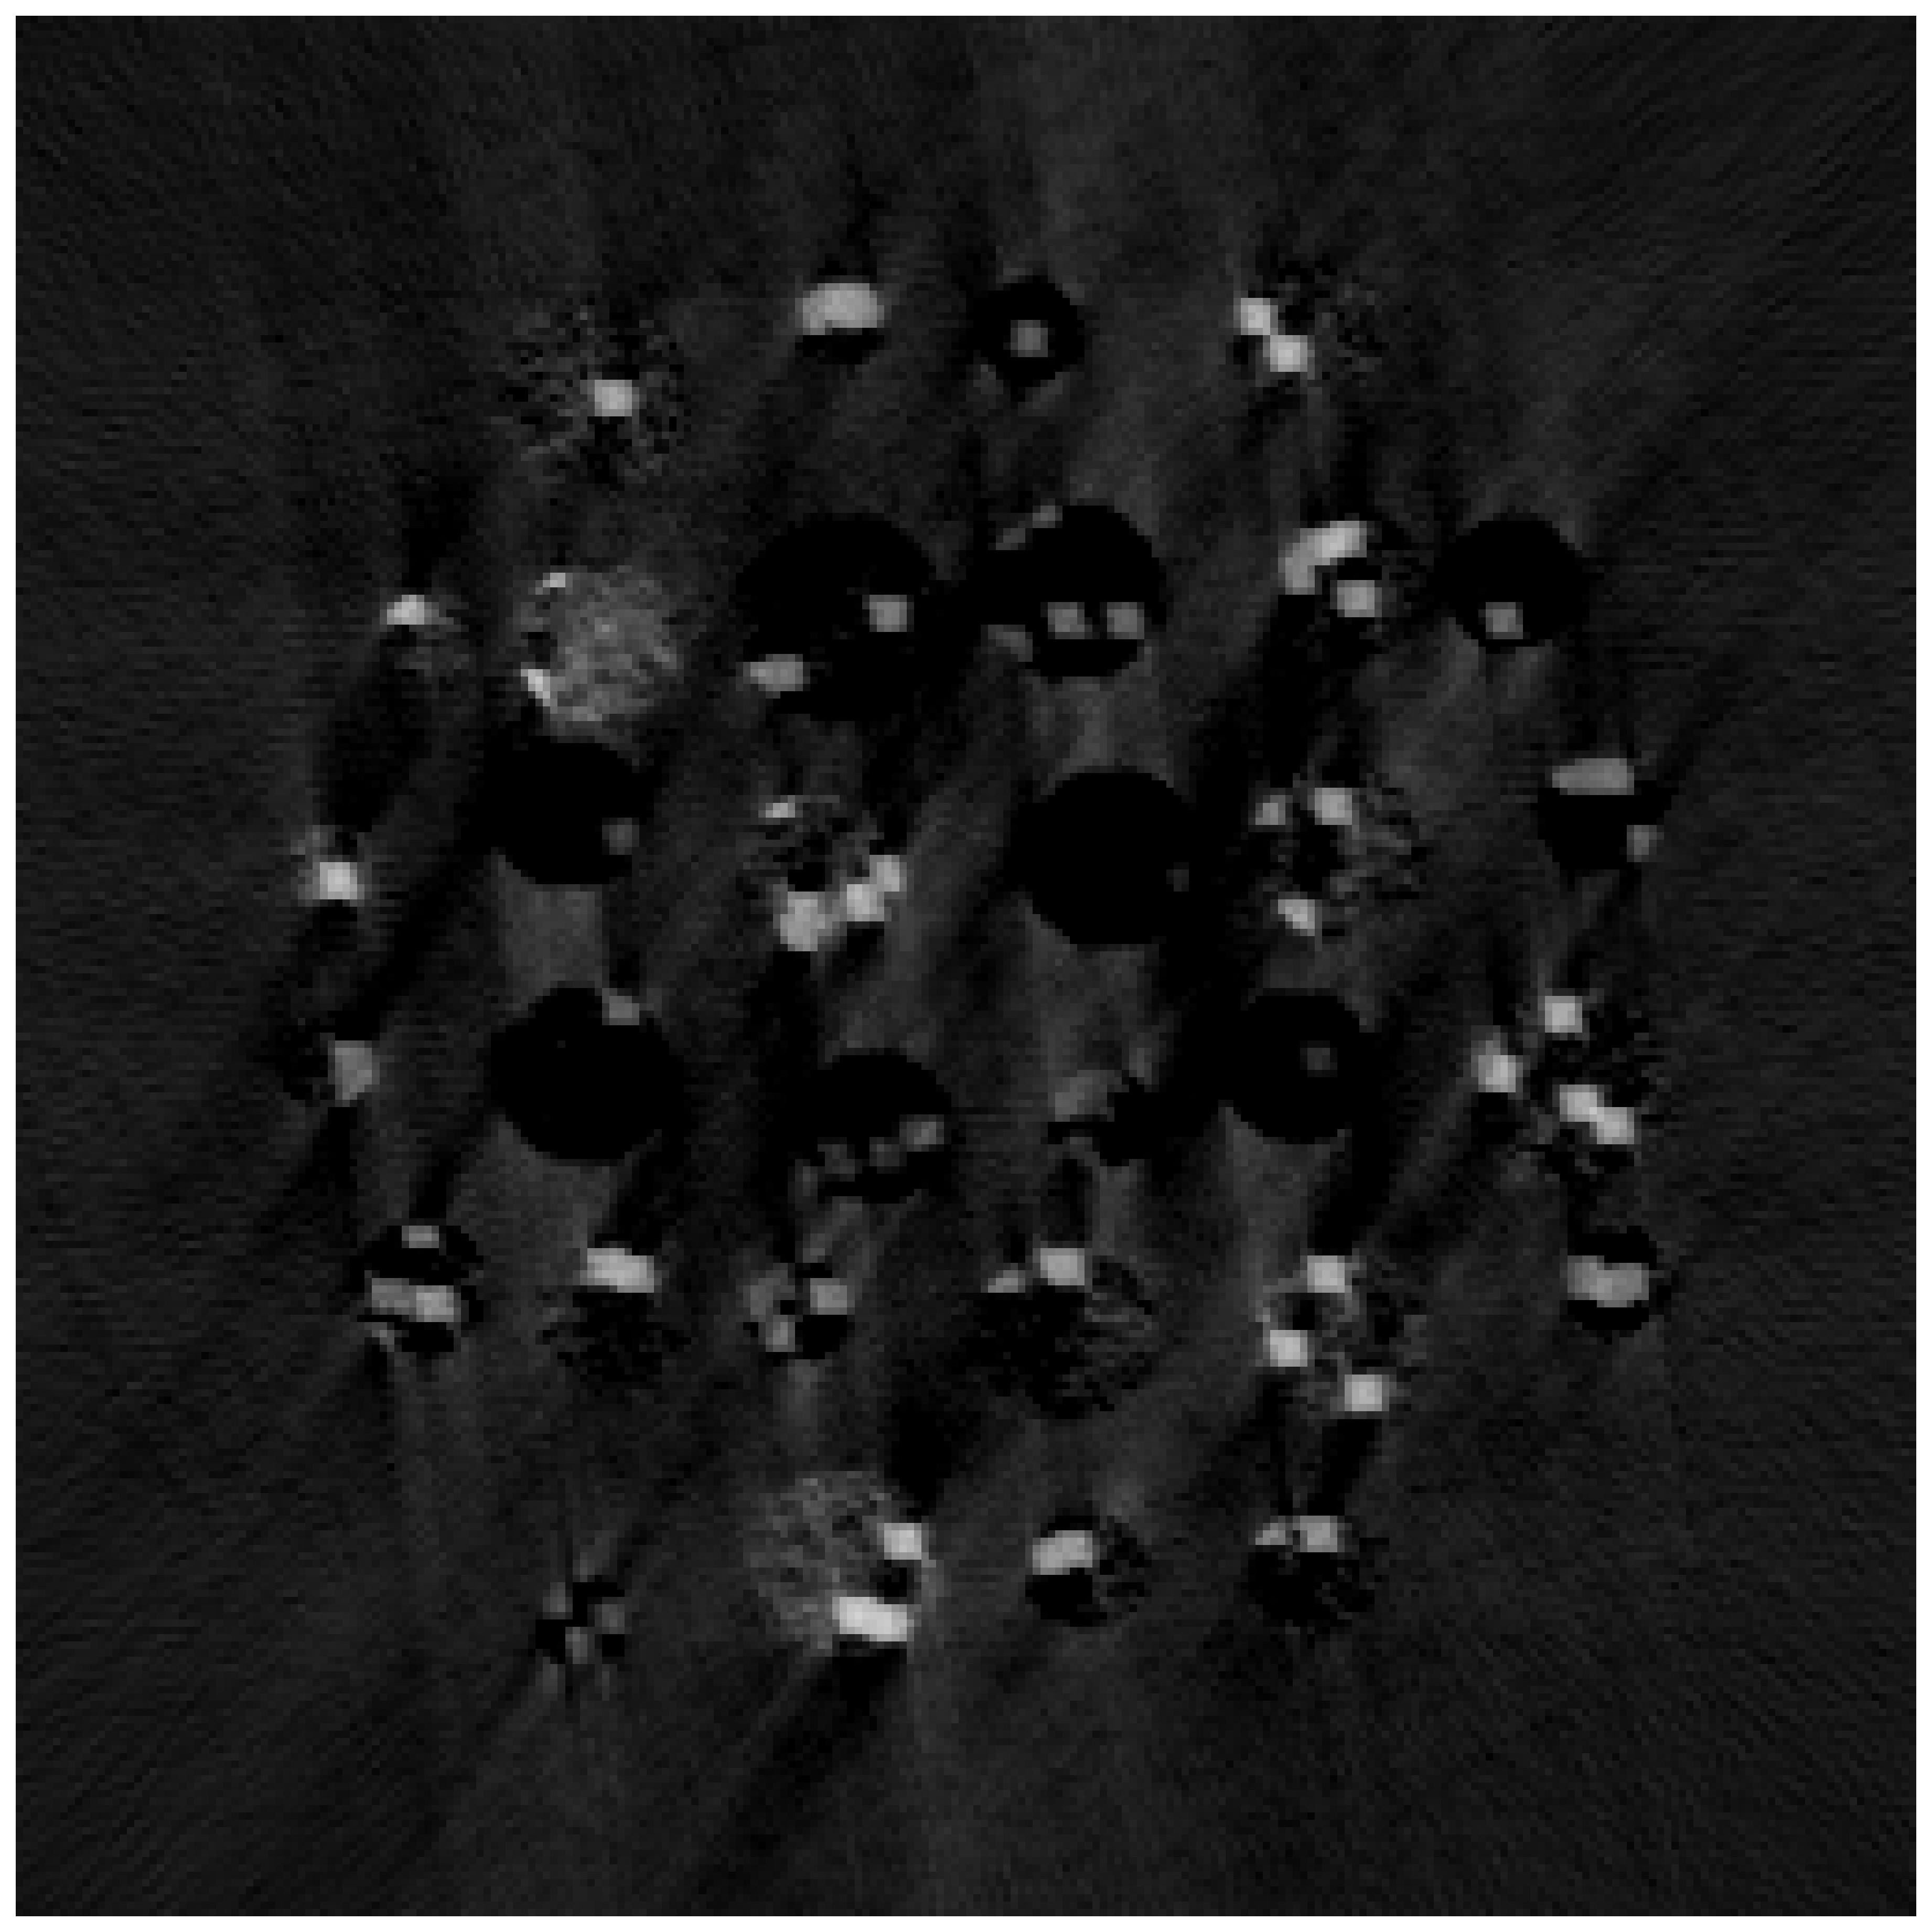
\includegraphics[width=0.15\textwidth]{graphics/holes_cad_tar.png}
\label{fig:holes_cad_tar}}
\caption{Understanding the action of the GAN on objects with internal defects not expected by the shape prior. (\ref{fig:holes_tar}) shows the target reconstruction, (\ref{fig:holes_gan}) shows the reconstruction with our method and (\ref{fig:holes_gan_tar}) shows the difference between (\ref{fig:holes_gan}) and (\ref{fig:holes_tar}). (\ref{fig:holes_cad}) shows the reconstruction with the shape prior and (\ref{fig:holes_cad_tar}) shows the difference between (\ref{fig:holes_cad}) and (\ref{fig:holes_tar}).}
\label{fig:images_with_holes}
        
\end{figure*}  

\end{document}